%!TEX root = ../dissertation.tex

\chapter{Origins of a complexity bias}
\label{chapter:origins}

\section{Introduction}

A universal property of languages is that they contain units of meaningful sounds---words---that vary in length. What accounts for this variability? That is, why is the word for ``can'' short but the word for ``calculator'' long? One class of explanations for this variability appeals to properties of the linguistic form itself, such as word frequency \cite{zipf1936} and predictability in linguistic context \cite{piantadosi2011a,mahowald2013info}. Our recent work has revealed an additional factor influencing word length: conceptual complexity. Across 80 natural languages, we find a bias for longer words to refer to conceptually more complex meanings ({\it complexity bias}; Chapter 2). This systematicity between word length and meaning challenges the long-held assumption that the relationship between form and meaning is entirely arbitrary \cite{saussure}.

In Chapter 4, we turn away from the question of what conceptual complexity is to the question of {\it why}: Why is there a complexity bias in the lexica of natural languages? We take as the central datum to be explained the bias in natural language for longer words to map onto more complex meanings (Studies 9 and 10 in Chapter 2).  To answer this question, we first consider the hypothesis space of the origins of a complexity bias in the lexicon. We then present a series of four studies that shed light on the relative likelihood of these different hypotheses.\footnote{Parts of this chapter are published in  Lewis, M. \& Frank, M. C. (2015). Conceptual complexity and the evolution of the lexicon. Proceedings of the 37th Annual Meeting of the Cognitive Science Society (p. 1138-1343). Austin, TX: Cognitive Science Society, and in,  Lewis, M., Sugarman, E., \& Frank, M. C. (2014). The structure of the lexicon reflects principles of communication. Proceedings of the 36th Annual Meeting of the Cognitive Science Society (p. 845-850). Austin, TX: Cognitive Science Society.}


\subsection{Hypotheses about the origins of a complexity bias}
The conceptual framework of  timescales is useful in understanding the space of hypotheses about the origins of a complexity bias. We assume that a complexity bias in natural language emerges at the timescale of language evolution. Critically, we also assume that the bias at the timescale of language evolution must have emerged---at some point---as the product of processes at shorter timescales, even if indirectly. In particular, we consider pressures at the timescales of language use and development. Below we describe four different hypotheses of pressures at shorter timescales that would, over time, lead to a complexity bias in the lexica of natural languages at the evolution timescale. These pressures are summarized in Table \ref{tab:bias_hypotheses}.


\hspace*{.3 cm}{ \it 1.\ The Efficient Naming Hypothesis.} To understand one variant of this hypothesis, consider the following fable: At the beginning of linguistic time, names were assigned to objects by length, starting with the shortest. Objects were named in the order that they were observed or as they became communicatively relevant. Since more frequent or communicatively-relevant objects  tended to be observed earlier, these objects received shorter names, relative to the less frequent objects that were encountered later.   The result is a language the contains a complexity bias in its lexicon.




\bgroup
\def\arraystretch{1.5}% 

\begin{table}[t!]
%\footnotesize
\centering
\begin{tabular}{l l l l l }
 \toprule
 \textbf{Hypothesis} &  \textbf{Pressure}& \textbf{\begin{tabular}[c]{@{}l@{}}Relevant\\Study\end{tabular}} \\
 \toprule
Efficient Naming Hypothesis   & \multicolumn{1}{p{8cm}}{Bias to name simple meanings  first {\it and} coin short words first.} & Study 1\\
Learning Hypothesis &  \multicolumn{1}{p{8cm}}{A lexicon with a complexity bias is more learnable.} & Study 2 \\
Memory Hypothesis & \multicolumn{1}{p{8cm}}{Speakers make memory errors by mis-remembering simpler meanings with shorter words.} & Study 3  \\
Pragmatic Hypothesis & \multicolumn{1}{p{8cm}}{ Speakers truncate simpler meanings with shorter words in order to facilitate communication.} & Study 4 \\

 \bottomrule
\end{tabular}
\caption{Summary of origin hypotheses and relevant studies.}
\label{tab:bias_hypotheses}
\end{table}
\egroup

%This story provides one possible account of the emergence of a complexity bias over the language evolution timescale.

This hypothesis posits two independent pressures operating at shorter timescales: The bias to name simple objects first and the bias to coin short words first. Both of these pressures could be due to pragmatic or cognitive demands. Importantly, however, the Efficient Naming Hypothesis suggests that the complexity bias in natural language is not directly reflected in psychological phenomena (the mind does not have a ``complexity bias"), but rather that the bias in natural language is epiphenomenal to psychological processes.

\hspace*{.3 cm}{ \it 2.\ The Learning Hypothesis.} 
A second possibility is that the pressure shaping the lexicon operates over the developmental timescale due to learning constraints: When learning the meaning of words, children are better able to learn a lexicon that tends to map complex meanings to long words and simple meanings to short words. Why might children have this bias? One possible account is that children have a bias to assume that there is resemblance between the form of a word and its meaning; that is, a bias for iconicity. There is a large literature suggesting that lexica of natural language indeed contain some degree of iconicity  \cite<see>[for review]{schmidtke2014phonological}. 

In addition, there is evidence suggesting that iconicity may facilitate word learning. For example, \citeA{imai2008sound} found that Japanese children were better able to acquire novel words that were iconically related their referents, relative to non-iconic words.\footnote{There is also some evidence to suggest that children may show the ``bouba-kiki`` effect \cite<the bias to map the word ``bouba" onto a curvy object, and ``kiki" onto a pointy object; e.g.,>{maurer2006shape}, but a recent meta-analysis of this literature suggests that this bias may not be robust in children \cite{lammertink2016}.} More broadly, in an analysis of early learned words, recent work suggests a relationship between the iconicity of a word and age of acquisition: In particular, more iconic words tend to be learned earlier \cite{perry2015iconicity}.

Thus, under this hypothesis, an iconic bias to map more complex meanings onto longer words exerts pressure over the timescale of development. Over language evolution, this learning pressure leads to a lexicon that facilitates learning by encoding a complexity bias. 

%This hypothesis is consonant with the broader proposal that language is shaped by learning pressures \cite{}

\hspace*{.3 cm}{ \it 3.\ The Memory Hypothesis.} This hypothesis posits that a cognitive bias, such as a bias for iconicity, exerts pressure on memory at the in-the-moment timescale. More specifically, a psychological bias for iconicity causes small changes in memory for complex phonological forms in the moment of language interaction, and  this  pressure leads to biases in linguistic transmission across generations. Over the course of language evolution, these psychological, synchronic biases result in a lexicon that magnifies this bias  \cite{griffiths2007language}. 

%Over time, this behavioral regularity might become a probabilistic rule,  becoming ``grammaticalized'' into the language. 

\hspace*{.3 cm}{ \it 4.\ The Pragmatic Hypothesis. } A final possibility is that humans are predisposed to consider the intentions of others \cite{tomasello2005understanding}. This predisposition leads to pragmatic reasoning. As argued by \citeA{horn1984}, one type of inference that might be guided by pragmatic reasoning is that a costlier (i.e.\ longer) utterance is more likely to refer to a more complex meaning, than a shorter one. Thus, under this hypothesis, domain-general pragmatic reasoning may underly an in-the-moment complexity bias. Over time, this in-the-moment bias may become grammaticalized, leading to a complexity bias in the lexicon. This possibility is consistent with other work showing that features of the lexicon also reflect principles of communication, like the structure of semantic space \cite{regier2007color,kemp2012kinship,piantadosi2012communicative}. 

%A second alternative is that the bias  is related to principles of communication.   As part of a broader theory of communication, \citeA{horn1984} suggested that a contrast in length between two phrases with the same denotational value implies a contrast in meaning, with the longer phrase getting the more unusual or complex meaning. Thus, the complexity bias  in the lexicon could reflect this in-the-moment communicative bias---

%A variant of this hypothesis is that an in-the-moment behavioral bias might be the product of both an underlying pragmatic inference and an overhypothesis about a complexity regularity in the lexicon. This possibility is similar to one account of a different, well-studied bias in word learning \cite{lewis2013b}: the mutual exclusivity bias. The mutual exclusivity bias is the tendency for children to map a novel word onto a novel object. In this work, we suggest that the mutual exclusivity behavior may emerge from both an in-the-moment pragmatic inference (the speaker would have used the known word to refer to a known object if that was the intended referent,  and so the novel word must refer to the novel object) and an overhypothesis about the structure of the lexicon (a 1-1 mapping between words and concepts).  We argued that processes at both timescales may jointly contribute to mutual exclusivity behavior. 

Importantly, these possibilities are not mutually exclusive with each other. In principle, all four of these hypotheses could simultaneously be correct and mutually enforcing. More likely, several of these might be true, perhaps with different weights. For example, speakers might have a bias for iconicity, which might lead to {\it both} memory errors and a learning bias. Furthermore, these different hypotheses may be causally related to each other: An iconic bias might lead to a pragmatic bias (i.e.\ if the speaker knows the listener is biased to assume that a long word refers to a complex meaning, then a helpful speaker will use that mapping). Indeed, there are a number of different hybrid accounts that can be derived from this space of possibilities. A final issue is how the in-the-moment bias---as evidenced by our novel word mapping experiments in Chapter 2---is accounted for. This issue is related to the account of the bias in natural language, though the accounts need not necessarily be the same. We return to this issue in the General Discussion.

In the present chapter, we appeal to data from four studies to shed light on the likelihood of these different hypotheses. In Study 1, we examine whether there is a complexity bias in a large sample of languages with primitive words. In Study 2, we ask whether this bias is present in language acquisition over the course of development. Finally, in Studies 3 and 4, we ask whether memory and pragmatic pressures might influence the emergence of a complexity bias in the lexicon. Taken together, we find that these data are most consistent with the Memory and Learning Hypotheses. 


%%%%%%%%STUDY 1-SWADESH%%%%%%%%
\section{Study 1a: Complexity norms for primitive words}
As a first step in exploring the origins of the complexity bias, we sought to replicate and extend our previous work suggesting that a lexical complexity bias was present in a diverse set of languages (Study 10, Chapter 2, pg.\ \pageref{ch2-10}). We also sought to test one prediction of the Efficient Naming Hypothesis. Recall that the Efficient Naming Hypothesis assumes that  meanings with high ``communicative need" should be named first, and that they should receive short labels. This thus predicts that words with high communicative need should not tend  to show a complexity bias cross-linguistically. Instead, they should all be named with relatively short words.

With these goals, we examined the complexity bias within a list of high communicative need words  developed by  \citeA{swadesh1955towards}, across a large sample of languages. We selected this list of words because it was developed explicitly to contain words that were conceptually primitive and therefore likely to have direct translation equivalents across languages. While similar, it is important for interpretation to note that the present study differs from Study 9 in Chapter 2 in several ways. First, the present study considers a much larger set of languages (80 vs.\ 1,037), but a smaller set of words (499 vs.\ 40). The words in the present sample are higher frequency and more conceptually primitive than the words in Study 9, and thus likely to have been borrowed from other languages. The words in the present sample also have less variability in word length. Finally, in the present study, we use a different metric of word length---phonetic code length rather than number of characters---to quantify length. This has the advantage of more closely resembling the spoken word, but nevertheless makes the two studies less comparable. This differences suggest we should be cautious in directly comparing the two samples. 

In Study 1a, we ask participants to rate the conceptual complexity of each of the word meanings on the Swadesh list, using a procedure similar to Study 9 in Chapter 2. Averaging across participants, we  estimate the conceptual complexity of each word in this sample.  In Study 1b, we then consider the translation equivalents of these words across 1,037 languages and ask how variability in conceptual complexity is related to word length in each language. If the Efficient Naming Hypothesis is correct, we should not expect to observe a robust complexity bias in this sample of words. Contra this prediction, we find a complexity bias in this large sample of languages, but smaller than in Study 10 with a different sample of words and languages.

%If the complexity bias in natural language observed in Study 9 in Chapter 2 is a robust phenomenon, we should expect the bias to extend to this new set of words and this broader sample of languages. 

\subsection{Method}
\subsubsection{Participants} We recruited 100 participants from Amazon Mechanical Turk.
\subsubsection{Stimuli}
We presented participants with subset of the word list developed by \citeA{swadesh1955towards}. This list was developed  for the purpose of inferring genetic relations between languages on the basis of their lexical similarity. The original list contains 100 meanings that are considered ``core vocabulary," and thus likely to be present in all languages (e.g., natural objects, colors, body parts). More recently, this list has been used in a project that aims to automatically generate language classifications on the basis of similarity between word lists \cite{brown2008automated}. In this project, it was found that comparable accuracy in classification could be achieved by using a subset of the original list, a 40-item list \cite{holman2008explorations}. The primary advantage of this smaller list is that translations are available for a much larger sample of languages. Thus, we adopted this 40-item word list in our work here (see Table~\ref{tab:swadeshwords} for full list of items). Each participant rated all 40 words from the  Swadesh word list. 

\begin{table}[t!]
\centering
\begin{tabular}{llllllll}
 \hline
blood  &  bone   &  breast   & come &    die    &  dog &     drink &  ear   \\
eye   &   fire   &  fish    & full   &  hand  &   hear &    horn  &   I  \\
knee  &   leaf   &  liver  &  louse  &  mountain  &name   &  new   &   night  \\
nose     &one    &  path     &person  & see    &  skin &    star  &   stone \\
sun  &    tongue  & tooth  & tree &    two      &water &   we    &   you     \\
 \hline
\end{tabular}
\caption{List of 40 Swadesh words.}
\label{tab:swadeshwords}
\end{table}

\subsubsection{Procedure}
We used the same norming procedure as in Study 9 in Chapter 2 (pg.\ \pageref{ch2-9}), with a few minor changes. In this version, participants were not given examples in the instructions and did not complete anchor trials.\footnote{A previous version of the experiment included instructions identical to Study 9 in Chapter 2. With these instructions, we find that there was limited variability in responses because all of the words were relatively conceptually simple, relative to the complex example and anchor item. Nevertheless, we also see a complexity bias in this sample, but smaller in magnitude ($r=0.32, p<.001$).} The full instructions seen by participants are presented below.  
\begin{quote}
In this experiment, you will be asked to decide how complex the meaning of a word is. A word's meaning is simple if it has few parts. A word's meaning is complex if it has many parts.
\end{quote}
For each word, we then asked ``How complex is the meaning of this word?,'' and participants indicated their response on a 7-pt Likert scale anchored at ``simple'' and ``complex.''

\subsection{Results and Discussion}
For each item, we calculated the mean complexity rating across participants ($M = .44$; $SD = 2.53$). We then used these ratings to estimate the complexity bias in the sample of words. We quantified word length in terms of number of characters. Consistent with previous studies, we find a positive correlation between word length and conceptual complexity ($r=0.51$, $p<.001$; Figure\ \ref{fig:study1a}). In Study 1b, we ask whether this relationship holds for a large sample of diverse languages.

\begin{figure*}[t!]
\begin{center}
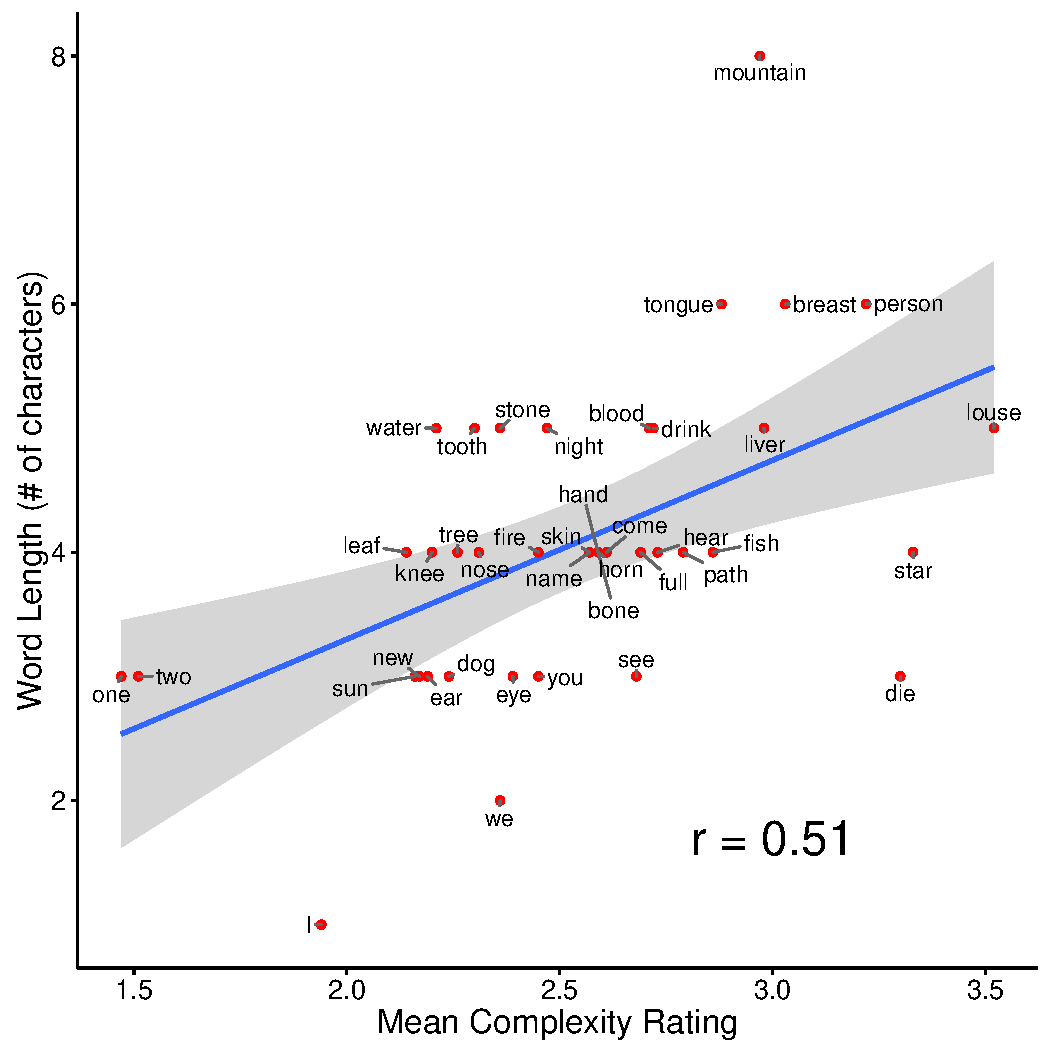
\includegraphics[scale = .6]{figs/chap4_1a.pdf}
\end{center}
\caption{Word length as a function of complexity norms for items in the 40-item Swadesh word list.}
\label{fig:study1a}
\end{figure*}


\section{Study 1b: Complexity bias for primitive words}

\begin{figure*}[t!]
\begin{center}
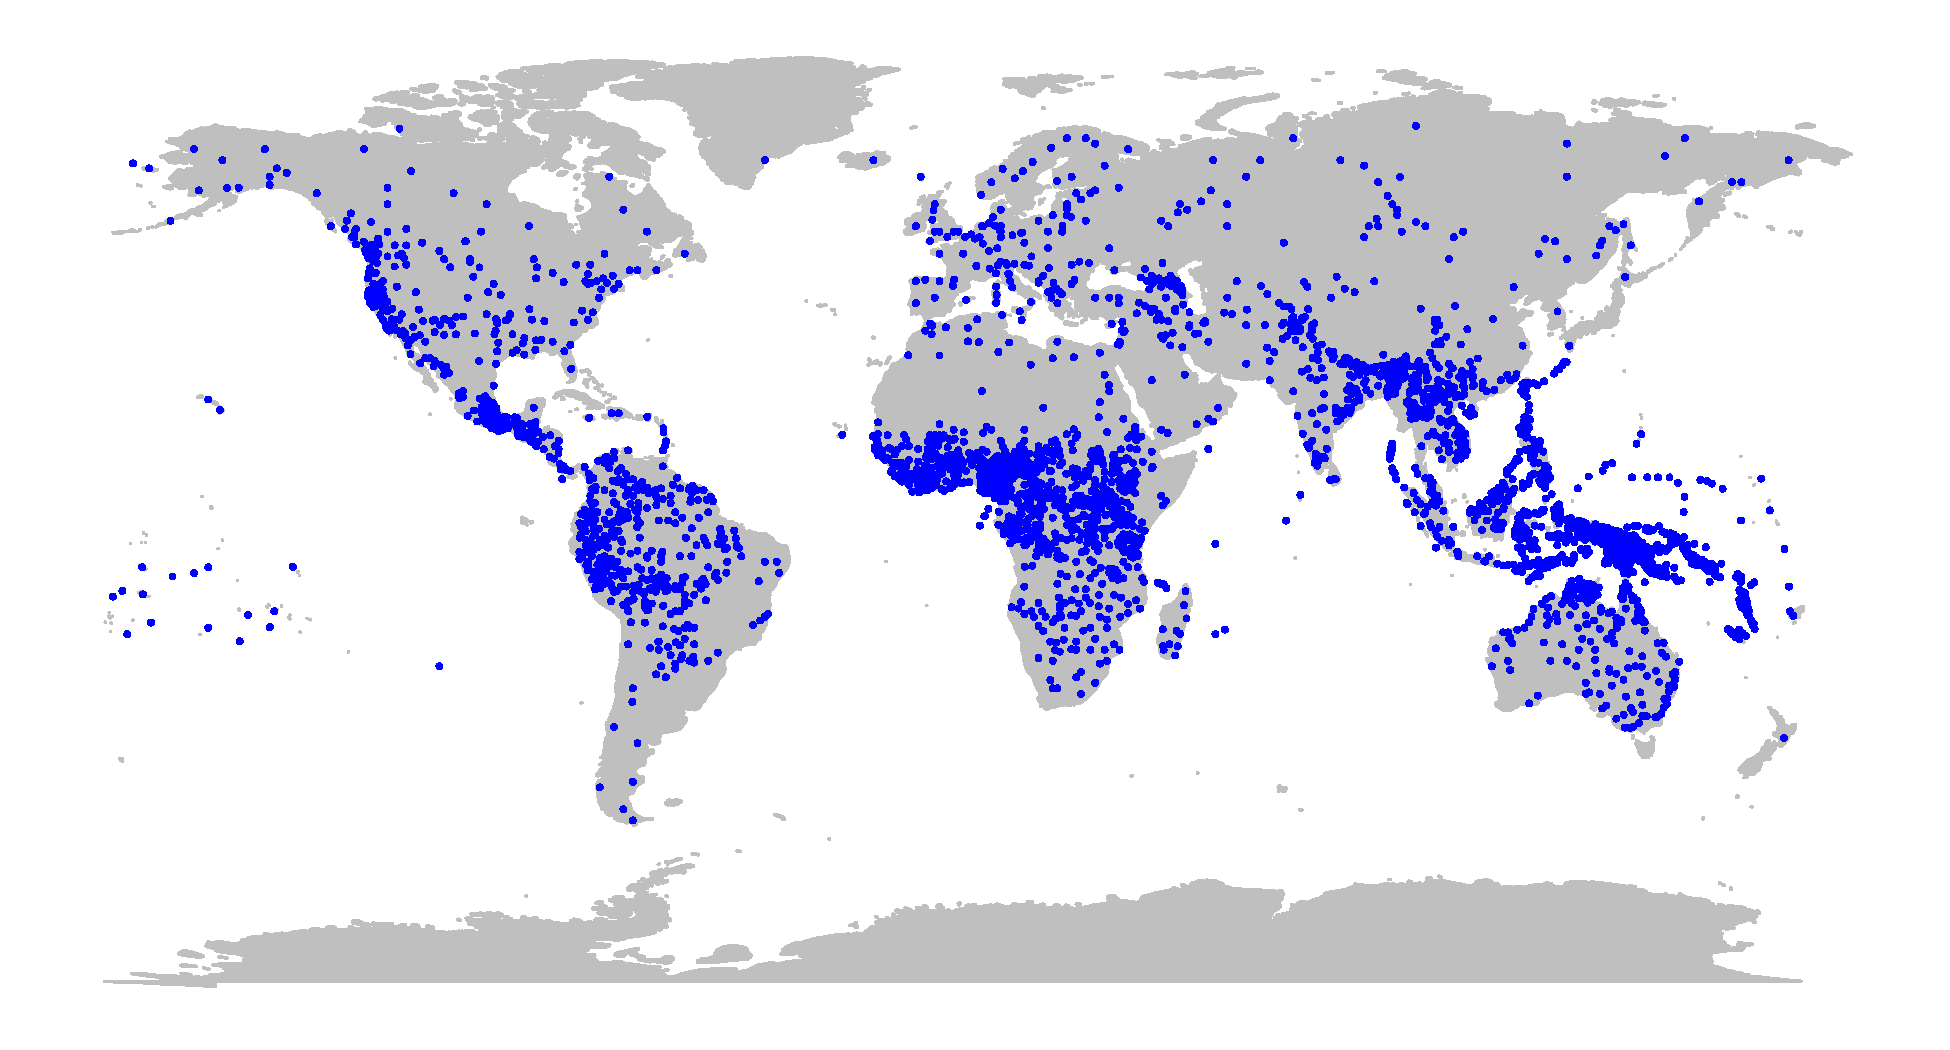
\includegraphics[scale = .45]{figs/chap4_1map.pdf}
\end{center}
\caption{Geographical distribution of languages in Study 1b. Each point corresponds to a language.}
\label{fig:study1b_map}
\end{figure*}

\subsection{Method}
To estimate the complexity bias cross-linguistically in this sample, we analyzed translations of the 40-item list in the  ASJP database \cite{asjp}. This database contains translations for the list of 40 words for 1037 languages from 261 distinct language families. The geographical distribution of the languages is shown in Figure\ \ref{fig:study1b_map}. For cross-linguistic comparability, this database transcribes words using a simplified version of International Phonetic Alphabet, called ASJPcode. In our analyses, we thus measure word length in terms of number of ASJP characters.

\subsection{Results}
For each language, we calculated the correlation between word lengths and complexity norms for the sample of 40 words. The distribution of correlations is shown in  
Figure\ \ref{fig:study1b} ($M = .12$; $SD = .17$). The magnitude of this correlation is affected slightly by the distribution of word lengths in each language, due to restriction of range. We corrected for this bias by calculating the maximum possible correlation between complexity ratings and word lengths in each language, and then normalizing the observed correlation by this maximum value. With this correction, the mean correlation was slightly larger ($M = .13$; $SD = .18$). 

\begin{figure*}[t!]
\begin{center}
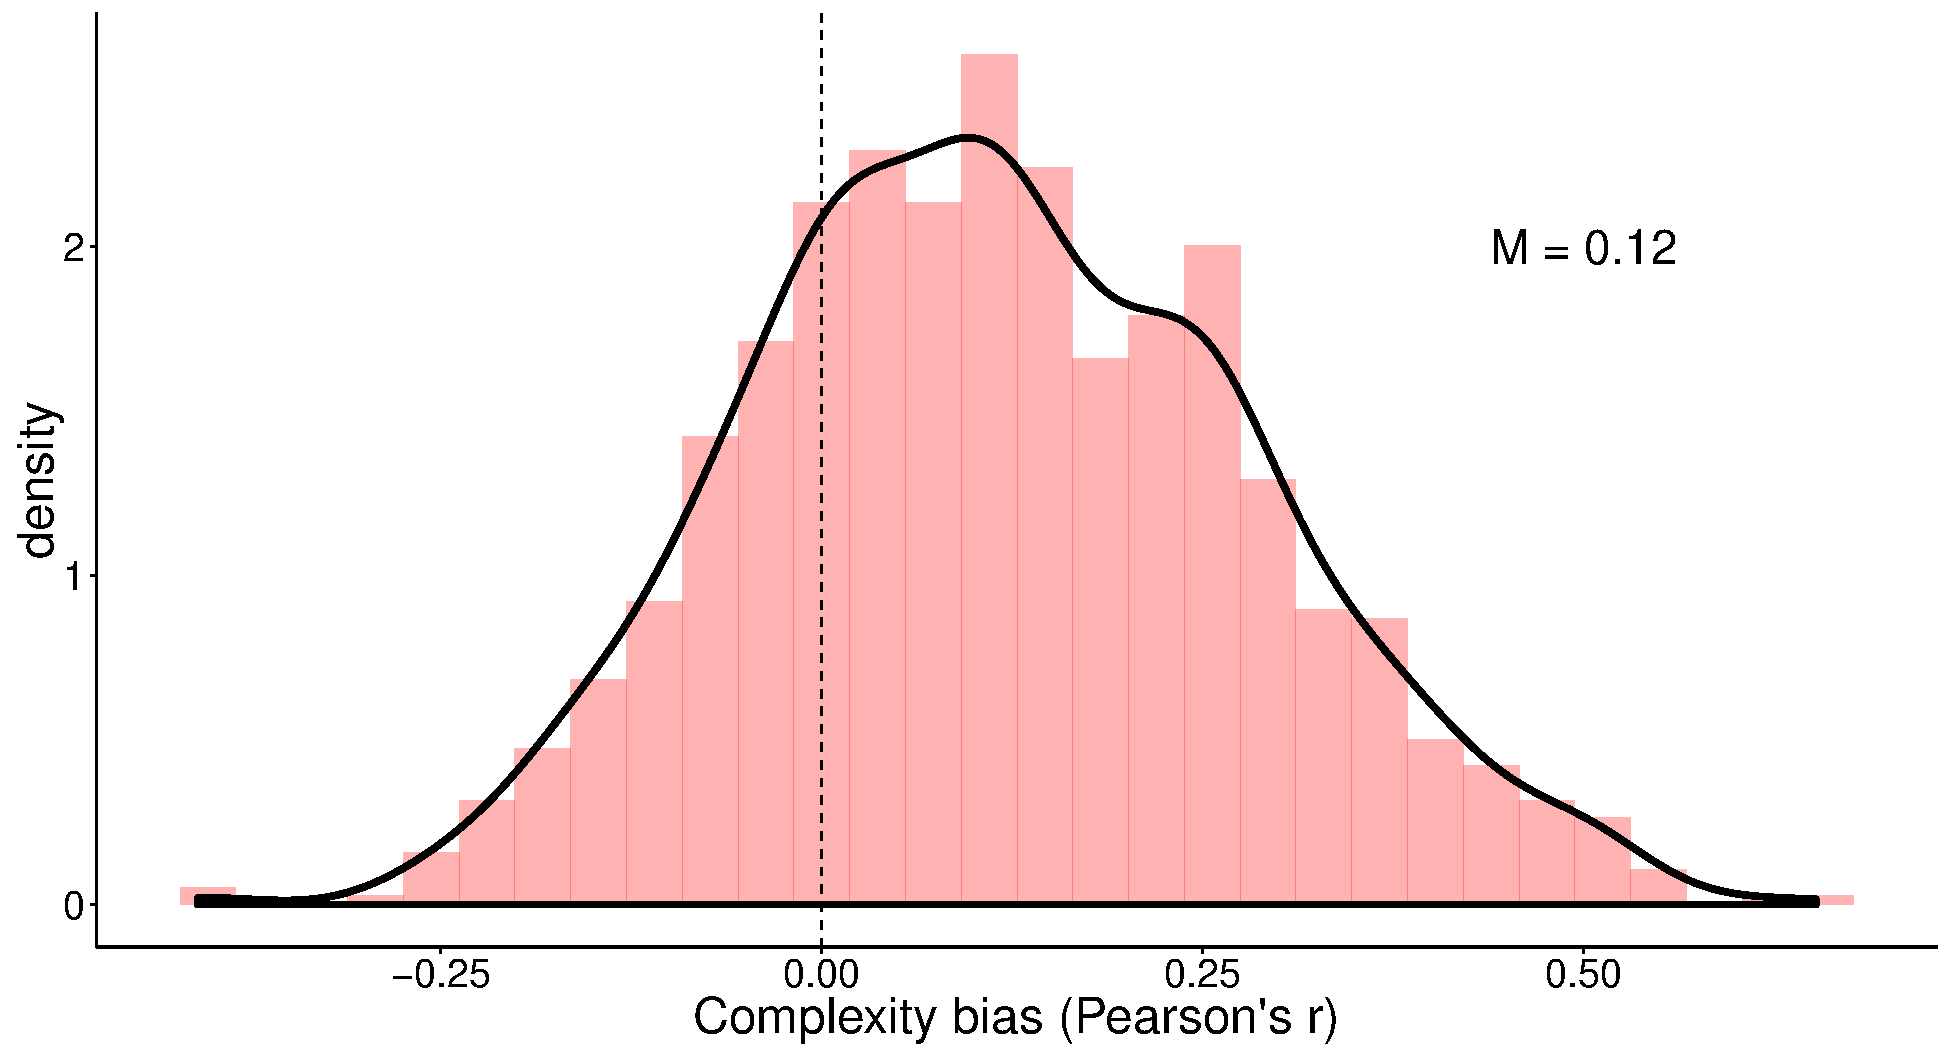
\includegraphics[scale = .35]{figs/chap4_1b.pdf}
\end{center}
\caption{For each language, we calculated the correlation coefficients between word length and complexity norms for the set of 40 words. This plot shows the distribution of correlation coefficients across all 1,037 languages. }
\label{fig:study1b}
\end{figure*}


Across languages,  the correlation significantly differed from zero ($ t(1036)= 22.87$; $p <.0001$).  To control for the non-independence of languages from the same linguistic family, we constructed a mixed-effect linear model predicting word length with complexity bias as a fixed effect. The random-effect structure included language and language family as both random slopes and intercepts.\footnote{The model specification was as follows: \texttt{word length $\sim$ complexity + (1 + complexity ~\textbar~language family) +  (1 + complexity ~\textbar~language)}. This was the maximal random effect structure that allowed the model to converge.}  The model showed a significant effect of complexity on length ($\beta = .18$, $t = 5.6$), suggesting that the complexity bias is present across a range of diverse languages.

We next compared these results to those observed in the sample of 499 words using Google Translate from Study 10 in Chapter 2 (pg.\ \pageref{ch2-10}). Across languages, the mean correlation between length and complexity norms was larger in the Study 10 sample ($M = .34$; $SD = .12$), compared to the current sample ($M = .12$; $SD = .17$). One potential source of this difference could be the degree of sampling error between the two samples: In the sample from Study 10, each language contained 499 words, whereas in the current sample, each language contains only 40 words. To control for this difference, we sampled 40 words from the words from Study 10 and recomputed  the mean correlation across languages. The down-sampled mean was comparable to the original  ($M = .34$; $SD = .17$). 

\subsection{Discussion}

In Study 1b, we replicate our finding from Study 10 in Chapter 2 with a larger and more diverse set of languages. In addition, the fact that we find this bias in a sample of high frequency, high communicative need words, provides some evidence against the Efficient Naming Hypothesis as the origin of the complexity bias in natural language.

As described above, the present study and Study 10 (Chapter 2) differ in many ways, making a direct comparison between the two samples difficult. Nevertheless, our best guess is that the overall mean correlation in the present sample is approximately .22  smaller than that in Study 10.  There are a couple possible explanations of this difference. The first is that a complexity bias is smaller in high frequency words, perhaps because high frequency words are most affected by other pressures in the linguistic system \cite{lieberman2007quantifying}. A second possibility is that because our norms were collected in English, we are better able to capture the conceptual complexity of Indo-European languages. The bias is thus smaller in the present study because the sample of language is more diverse.  This second possibility seems unlikely, however, given that the present set of meanings are unlikely to vary dramatically across languages. 


%%%%%%%%STUDY 2a - ELISE %%%%%%%%
\section{Study 2a: Complexity bias in preschoolers }

% we ask whether conceptual complexity  plays a role in language acquisition. 

In Study 2, we explore a second hypothesis about the origin of the complexity bias: The Learning Hypothesis. The Learning Hypothesis posits that a complexity bias in young children facilitates learning of the lexicon. If true, this predicts that young children should show a complexity bias in learning the meanings of new words. In Study 2a, we present preschoolers with a task nearly identical to the novel word mapping experiments conducted with adults in Chapter 2. On each trial, children are presented with two novel objects and a novel word that is either short or long. Critically, the two object alternatives differ in complexity. If children have a bias to assume that long words refer to complex referents, and simple words refer to simple referents, we should expect to observe this bias in their guesses of the word's meaning.  We find evidence consistent with this prediction in the older children in our sample. 

\subsection{Methods}
\subsubsection{Participants} We recruited 108 children (60 girls) from a nursery school at Stanford University and the San Jose Children's Discovery Museum (36 3-year-olds, $M$= 3;8; 36 4-year-olds, $M$= 4;5; 36 5-year-olds, $M$= 5;5). 
\subsubsection{Stimuli} 
The object stimuli were the novel, real objects used in previous experiments (Fig.\ \ref{fig:realobjs};  pg. \pageref{novelrealobjs}). The linguistic stimuli were novel words either 2 or 4 syllables long (e.g., ``bugorn'' and ``tupabugorn''), as in previous experiments.

\subsubsection{Procedure} 
Children first completed a training phase to gain familiarity with  the iPad's touchscreen. They were then introduced to a puppet named Furble and told that  ``he speaks a different language from us. He has some toys that will look familiar, but he has lots of funny-looking toys, too. I need you to help me pick Furble's toys. Furble's going to say a word, and you're going to pick which toy you think the word is for." Children were then shown a display with two images, and the experimenter  asked the child in child-directed prosody to select a referent using one of three naming frames (``Can you find the [label]?,'' ``Where's the [label]?,"  or ``Can you pick the [label]?").

We manipulated word length within participants. Children completed 12 trials: four trials with long words, four trials with short words, and four trials with familiar words. Familiar word trials involved a familiar word and two familiar objects. These were included to familiarize children with the task of reference selection. Order of trials was randomized with the constraint that two familiar trials always appeared first.

\subsection{Results}
Figure\ \ref{fig:study2} illustrates the proportion of children selecting the complex referent in the short and long word conditions. Five percent of trials were excluded in cases where the child had difficulty operating the iPad, or where there were technical difficulties.  Across the three age groups, a complexity bias emerged only in 5-year-olds.

\begin{figure*}[t!]
\begin{center}
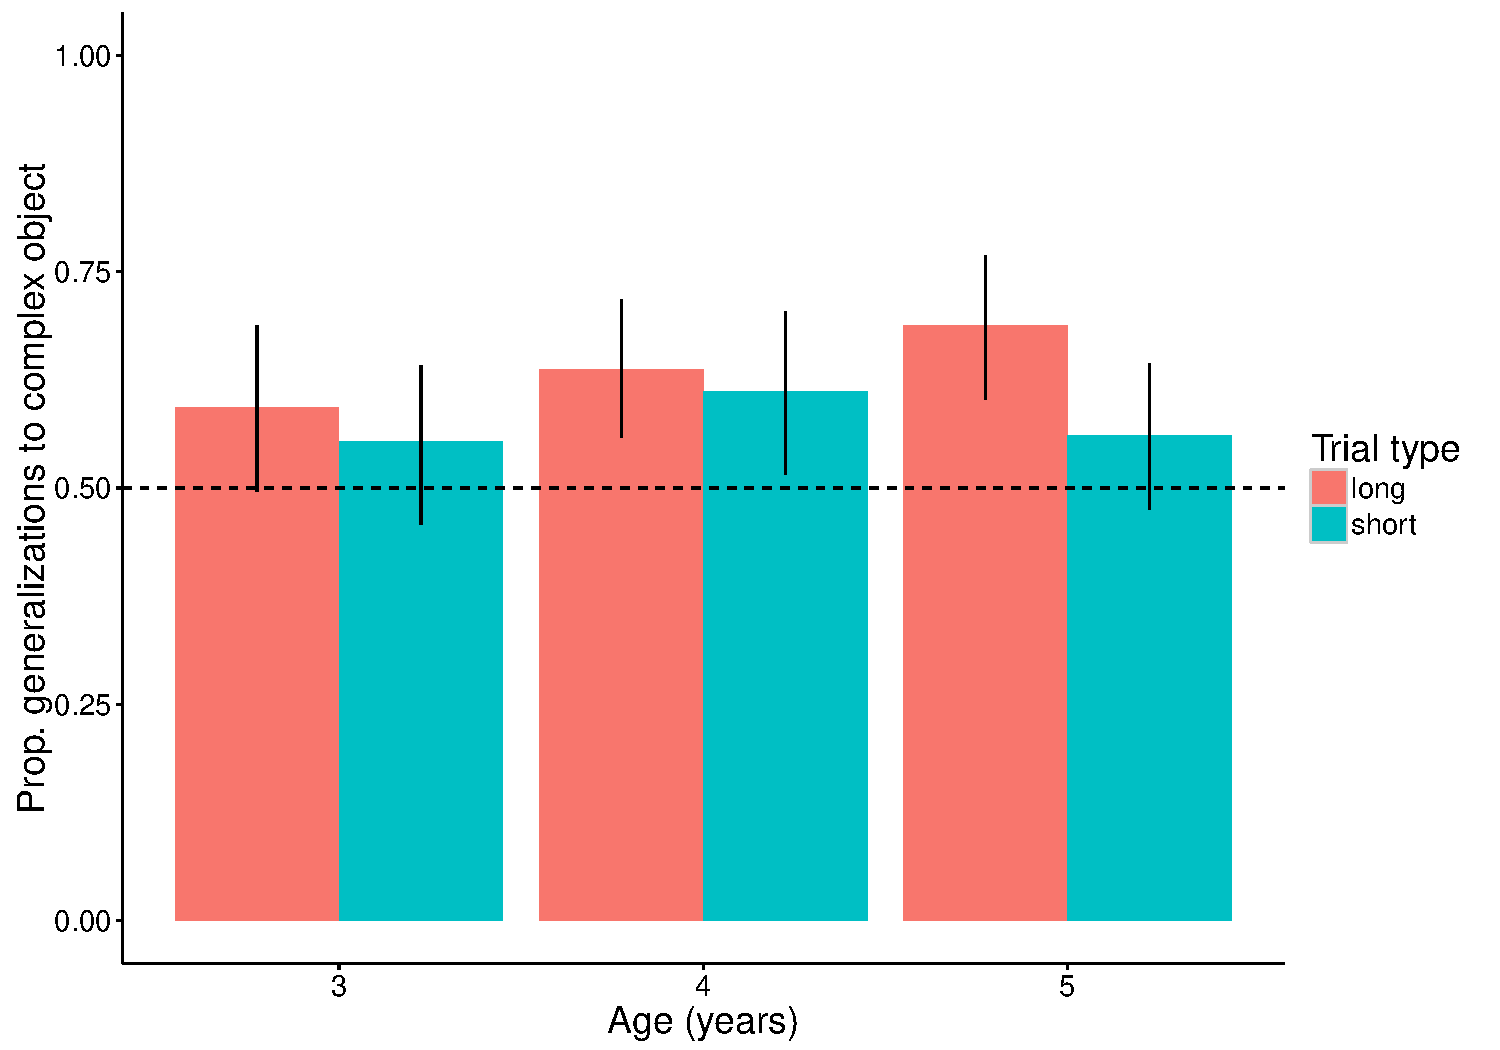
\includegraphics[scale = .5]{figs/chap4_2.pdf}
\end{center}
\caption{Mean proportion selections to complex object for children in Study 2. Error bars represent  95\% CIs as computed via non-parametric bootstrap. }
\label{fig:study2}
\end{figure*}

To test the reliability of this difference, we ran a generalized linear mixed model predicting object selection as an interaction between condition (long or short word) and age with random effects of participant and trial number. There was a main effect of age ($\beta=-0.40$, $p <.01$), indicating that children were overall more likely to select the complex  referent with increasing age. There was also a reliable interaction between age and condition ($\beta=0.38$, $p <.05$). The effect of condition was not significant.

We  ran a series of paired {\it t}-tests to examine response differences between conditions for each age group (3s, 4s, and 5s). There was a reliable difference between conditions for the 5-year-old age group ($t(35) =2.35, p<.05$, $d=.48$), but not the younger groups. 

%These results suggest that older, but not younger,
\subsection{Discussion}
These results provide some tentative evidence consistent with the Learning Hypothesis: When faced with novel words, older  preschoolers have an adult-like bias to map longer words onto more complex referents. Nevertheless, it is puzzling why the younger children in our sample, who are likely to be learning many new words, did not show the bias. This null effect may reflect a true absence of a complexity bias in young children. One possible explanation of this absence is that the bias is pragmatically driven and younger children do not have yet have competency in this type of reasoning. This possibility is consistent with a body of work on children's interpretation of scalar implicatures that suggests that reasoning in this age group is fragile and highly sensitive to aspects of the task \cite<for a review, see>{horowitz2016the-trouble}. Alternatively, this bias may simply be smaller in this population and we do not have the power to detect it in the current study. The present data do not allow us to distinguish between these two possible explanation of the null finding in the younger children.. 

Minimally, however, these data  suggest that relatively young children show a complexity bias, and thus that conceptual complexity may play a role in word learning,  as predicted by the Learning Hypothesis.

%%%%%%%%STUDY 2b - CDI%%%%%%%%
\section{Study 2b: Conceptual complexity and the early vocabulary}
In Study 2b, we explore two additional predictions of the Learning Hypothesis:  (1) Children's early vocabulary should contain a complexity bias, and (2) the conceptual complexity of a word's meaning should influence the ease with which words are learned. In particular, we predict that if conceptual complexity is relevant in acquisition, then children should tend to acquire words with simpler meanings before those with more complex meanings.

To test these predictions, we analyzed the conceptual complexity of words in children's early vocabulary using the MacArthur-Bates Communicative Development Inventory \cite<CDI;>{fenson2007}, a parent-report checklist of children's word knowledge. We find evidence consistent with both predictions: Early vocabulary contains a complexity bias, and children tend to learn conceptually simple words before more complex ones.

\subsection{Method}
\subsubsection{Participants} We recruited 252 participants from Amazon Mechanical Turk.
\subsubsection{Stimuli} Participants were presented with a subset of words from the Words and Sentences Form of the CDI \cite{fenson2007}. We excluded items that were onomatopoeic sounds (e.g.\ ``moo") or contained more than one word (e.g.\ ``rocking chair"). The final list contained 625 items. 
\subsubsection{Procedure} We used the same norming procedure as in Study 1a, except that participants were given an example of a simple and complex meaning in the instructions and  rated two anchor words (``ball" and ``motherboard;" as in Study 9 in Chapter 2). Each participant rated a sample of 40 words. 

\subsection{Results and Discussion}
The mean complexity rating for the anchor words suggested that participants  interpreted the scale as intended (``ball:" $M =1.33$; $SD = .93$; ``motherboard:" $M = 5.86$; $SD = 1.66$). Each of the 625 target words  was rated by an average of 16 participants, with a mean complexity rating of 2.77 ($SD = .77$). We next analyzed how these by-item complexity norms were related to two factors: Word length (Analysis 1; complexity bias) and age of acquisition (Analysis 2). 

\begin{figure}[t!]
\begin{center}
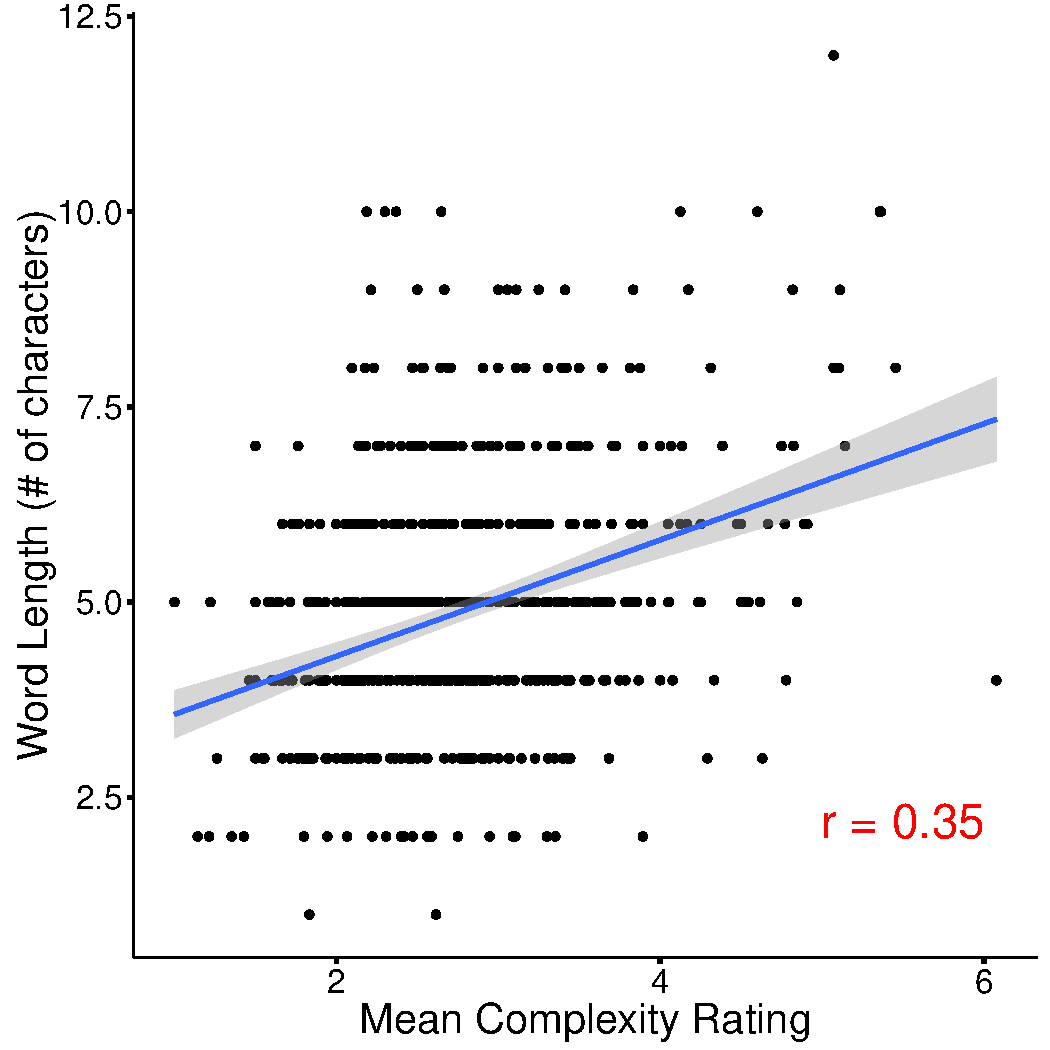
\includegraphics[scale = .5]{figs/chap4_3.pdf}
\end{center}
\caption{Word length as a function of complexity norms for all items on the CDI Words and Sentences Form. In child vocabulary, words that are conceptually more complex tend to be longer.}
\label{fig:study3}
\end{figure}


\subsubsection{Analysis 1: Complexity bias in acquisition}
As in previous studies, there was a reliable correlation between word length and complexity norms: Words whose meanings were rated as more complex tended to be longer ($r=0.35, p<.001$; Figure \ref{fig:study3}). To evaluate this relationship controlling for frequency, we fit an additive linear model predicting word length with frequency (log) and complexity. We used an existing metric of spoken word frequency derived from CHILDES, a child-directed corpus \cite{braginsky2016from}. This measure was only available for the subset of words (Words and Gestures Form; $n = 391$), and thus we only conducted this control analysis on this subset. In this analysis, both complexity ($\beta=.68$, $t=7.51$, $p <.0001$) and spoken word frequency ($\beta=-.52$, $t=-10.44$, $p <.0001$) were reliable predictors of word length, suggesting that complexity accounted for variability in word length over and above spoken frequency.

We also examined whether a complexity bias was present in acquisition cross-linguistically. We analyzed translation equivalents of the set of words on the Words and Gestures CDI form, taken from \citeA{braginsky2016from}. We analyzed  languages present in all three datasets thus far studied---the Google words (Chapter 2, Study 10), the Swadesh words (Chapter 4, Study 1), and the present set of CDI words---leaving us with a total of seven languages, including English. All seven languages showed a complexity bias. In addition, there was a positive correlation across languages between the CDI words and the Google words ($r = .30, p = .52$), and between the CDI words and the Swadesh words ($r = .59, p = .30$), though neither of these correlations were statistically significant. Figure \ref{fig:synthesis4} shows the correlation coefficient for each language, in each dataset, as well as the correlation partialing out log spoken frequency. While these data represent only a small sample of languages, they are suggestive that the bias is stable across different samples of words.

\begin{figure}[t!]
\begin{center}
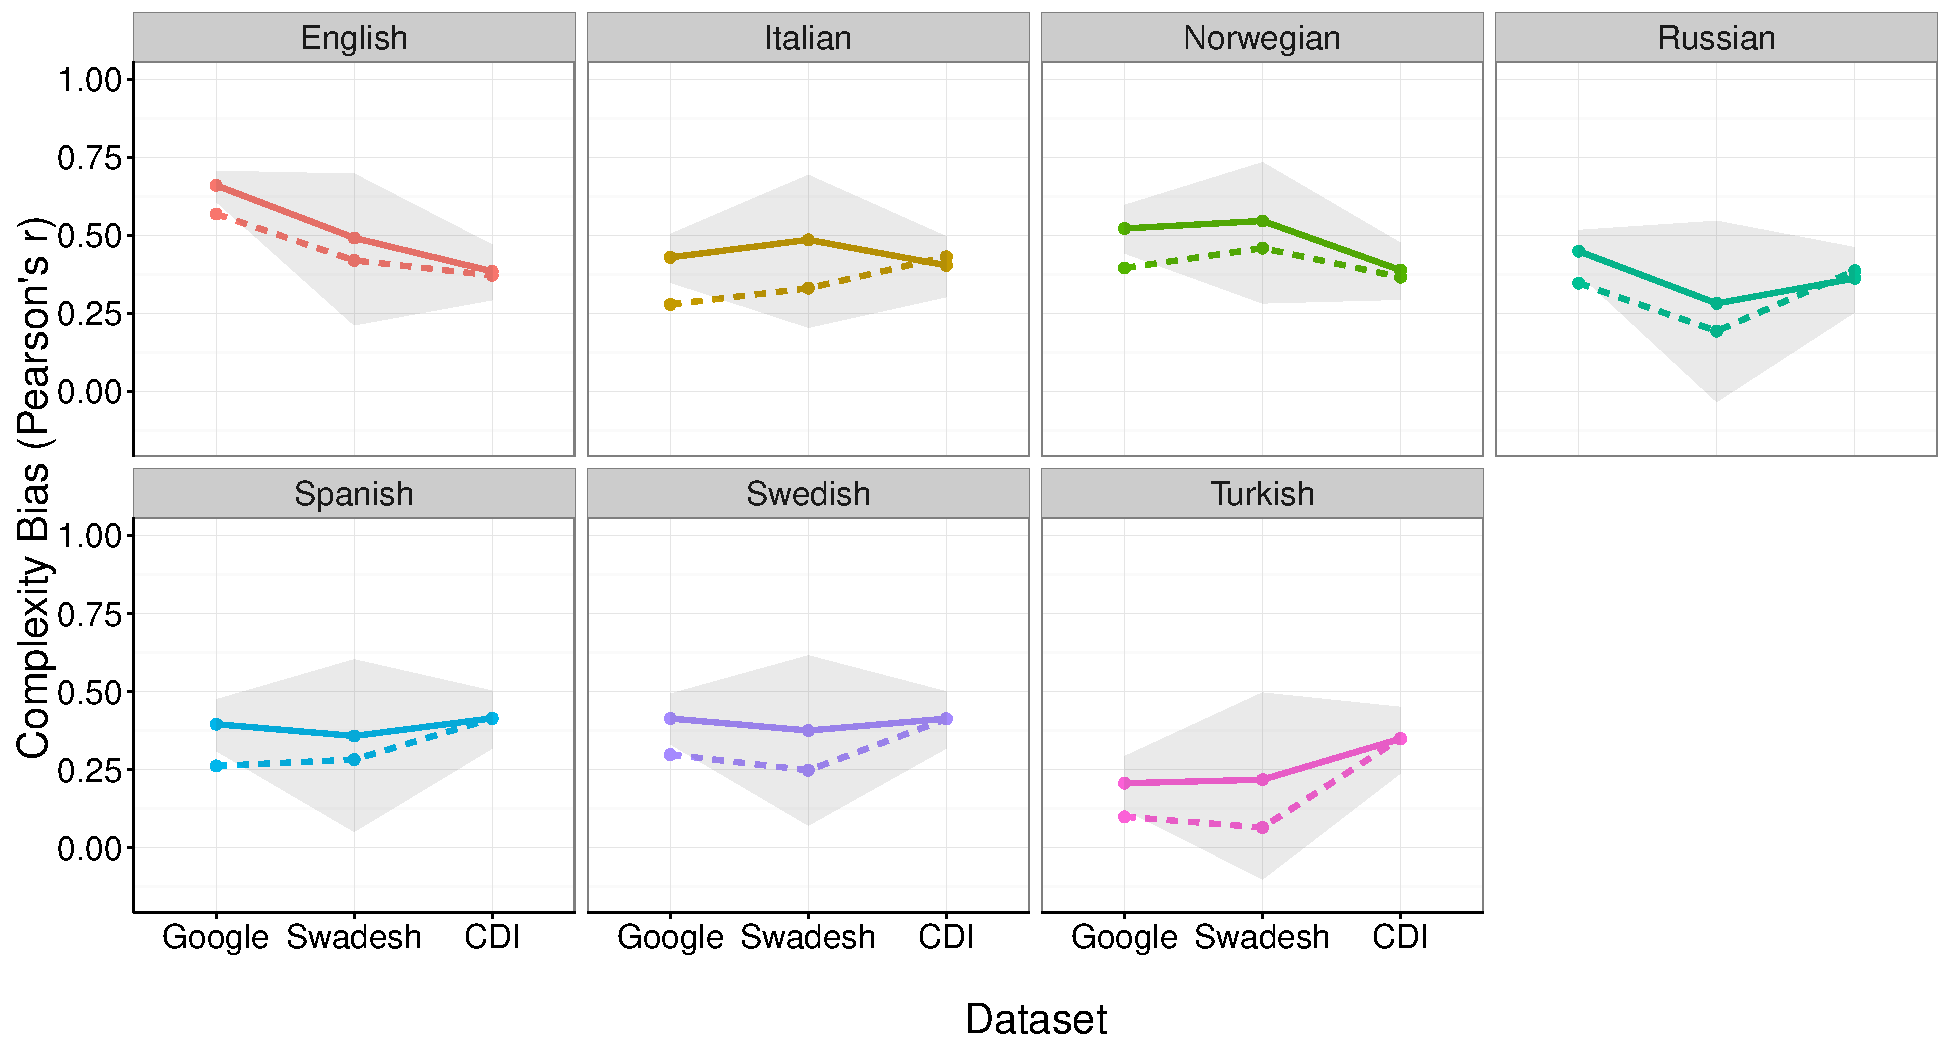
\includegraphics[scale = .47]{figs/chap4_synthesis2.pdf}
\end{center}
\caption{Pearson coefficients between word length and complexity norms across three samples of words (Google, Ch.\ 2, Study 10; Swadesh, Ch.\ 4, Study 1; and CDI Words and Gestures Form, Ch.\ 4, Study 2) for seven different languages. Solid lines show simple correlation between word length and complexity, and dashed lines show the correlation partialing out the effect of log spoken frequency. Ribbons show the parametric 95\% CI for the simple correlation. }
\label{fig:synthesis4}
\end{figure}




\subsubsection{Analysis 2: Conceptual complexity as a predictor of age of acquisition}
In Analysis 2, we asked whether the complexity of a word's meaning predicted its age of production. We estimated the age of acquisition of a word using the measures from \citeA{braginsky2016from}. In this work, age of acquisition for each word is estimated based on a database of CDI parent-report vocabulary forms  from over 42,000 children \cite<Wordbank;>{frank2016wordbank}. Using this database, \citeA{braginsky2016from} estimated the age of acquisition of each word as the age at which at least 50\% of children produce the word. In the present analysis, we find a reliable correlation between mean age of production of a word and conceptual complexity ($r=.20, p<.0001$; Figure \ref{fig:study3aoa}): Words that are conceptually more complex tend to be produced later in development. 

\begin{figure}[t!]
\begin{center}
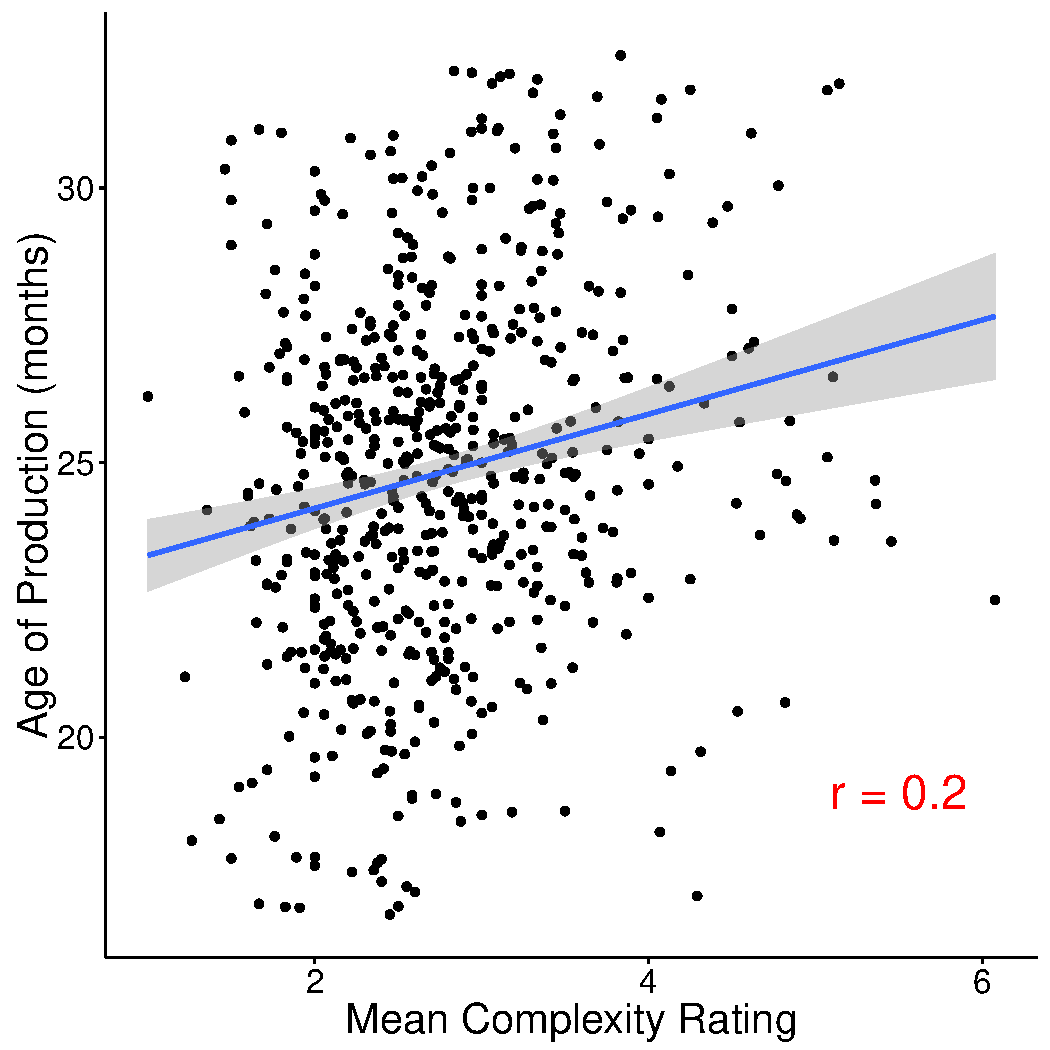
\includegraphics[scale = .5]{figs/chap4_aoa.pdf}
\end{center}
\caption{Age of production as a function of conceptual complexity. Words that are conceptually more complex are produced later.}
\label{fig:study3aoa}
\end{figure}





Importantly, however, the age of acquisition of a word is predicted by many other factors, such as the length of the word itself. Thus, we next asked whether complexity is an independent predictor of variance in the age of acquisition of words. We fit an additive linear model predicting age of production of each word with complexity, and six control variables from \citeA{braginsky2016from}: Word length, spoken frequency, concreteness (abstract vs.\ concrete), babiness (degree of association with infancy), valence (happy vs.\ unhappy), and arousal (excited vs.\ calm).  Again, these control variables were only available for the subset of words on the Words and Gestures Form ($n = 391$), and so we conducted the control analysis only on this subset. All variables were reliable predictors of age of acquisition, except word length and valence. Model fits are shown in Table \ref{tab:aoapred}. This suggests that the complexity of a word's meaning many influence the ease with which a word is acquired in language production: More complex words are produced later.

% latex table generated in R 3.3.0 by xtable 1.8-2 package
% Wed Oct 26 11:31:00 2016
\begin{table}[t!]
\centering
\begin{tabular}{rrrrr}
  \hline
 & Estimate & Std. Error & t-value & p\\ 
  \hline
(Intercept) & 8.7866 & 2.0437 & 4.30 & $<.0001$ \\ 
  complexity & 0.5154 & 0.2552 & 2.02 & $<.05$ \\ 
  word length & -0.1626 & 0.1450 & -1.12 & 0.26\\ 
  log frequency  & -1.2439 & 0.1801 & -6.91 & $<.0001$ \\ 
  concreteness & -1.0974 & 0.2502 & -4.39 & $<.0001$\\ 
  babiness & -0.4313 & 0.0864 & -4.99 &$<.0001$\\ 
  valence & 0.2037 & 0.1587 & 1.28 & 0.20 \\ 
  arousal & 0.4159 & 0.2037 & 2.04 &$ <.05$ \\ 
   \hline
\end{tabular}
\caption{Additive linear model predicting age of production of a word with conceptual complexity, and six other control variables. Complexity is a reliable predictor of age of acquisition}
  \label{tab:aoapred}
\end{table}

In summary, in acquisition we find that (1) older preschoolers have an in-the-moment complexity bias, (2) children's early vocabulary shows a complexity bias across seven different langauges, and (3) complexity predicts the age of acquisition of new words. Taken together, these findings are consistent with the possibility that the  complexity bias observed in natural language may be influenced by a learning bias in children over the course of language acquisition, as predicted by the Learning Hypothesis. 


%%%%%%%%STUDY 3%%%%%%%%
\section{Study 3: Iterated learning in a solo memory task}

In Study 3, we directly explore the Memory Hypothesis as a possible explanation of the origin of the complexity bias in natural language. The Memory Hypothesis posits that speakers mis-remember word forms in a way that is consistent with a complexity bias (shorten simple forms and lengthen complex forms) and, over time, these errors influence the structure of the lexicon.  To test this hypothesis, we use the iterated learning paradigm, a recently-developed method for studying language change in the lab \cite<e.g.,>{kirby2008cumulative,reali2009evolution,smith2010eliminating}. The critical feature of this paradigm is that the learning output of one speaker becomes the learning input for a new speaker. This paradigm allows us to examine the evolution of a language for a ``chain'' of speakers learning and transmitting a language. The dynamics of these chains serve as an approximation of the dynamics of generations of children acquiring and then transmitting language to future generations. 



A secondary goal of this study is to examine how psychological pressures influence the structure of the lexicon, independent of conceptual pressures.  Forms that are difficult to remember are unlikely to survive in the language  \cite{christiansen2008}, and there may be an additional communicative pressure for economy of expression \cite{zipf1949human}. Both of these pressures might lead to a preference for shorter words over longer, harder-to-produce words, biasing the ultimate structure of the lexicon towards shorter, more memorable words. 

We used an iterated learning paradigm to study the dynamics of these two aspects of the lexicon: how  words change over the course of language evolution and how conceptual complexity interacts with these changes.\footnote{For ease of measurement, we operationalize word length in terms of number of orthographic characters. However, this measure is highly correlated with measures of length with greater psychological reality, such as phonemes and morphemes (see Chapter 2).} As predicted, we find that forms in the lexicon converge to a more stable state and that a complexity bias emerges in the mappings between words and referents. We also find that the complexity bias is attenuated over time. A post-hoc analysis suggests that this change in the complexity bias over time is related to the degree of cross-generational change in the lexicon.


\subsection{Method}

Given existing evidence that a complexity bias is present in one-shot learning games (Chapter 2),  our experiment was designed to test how conceptual pressures influenced the lexicon over the course of transmission. We asked speakers to learn a novel language that contained meanings of varying complexity and words of varying length. Critically, the language we asked participants to learn contained no systematic relationship between complexity and word length. After studying these mappings, participants were asked to recall them. The measure of interest was the relationship between the errors participants made and the complexity of the referent. If participants show a complexity bias, they should be more likely to add characters for more complex objects and remove characters for less complex objects. 

This design characterized the first generation of our task. We then gave the labels that participants produced in the test phase of this first generation to a new set of speakers and asked them to complete the exact same task. We iterated 7 generations of this task in total.


\subsubsection{Participants} 

We recruited 350 participants from Amazon Mechanical Turk. Each generation was composed of 50 learners.

\subsubsection{Stimuli}

The referents were a set of 60 real objects that did not have common labels associated with them. These objects had been normed for their complexity in previous work (Study 4, Chapter 2; Fig.\ \ref{novelrealobjs}). Norms were obtained by asking participants to indicate ``How complicated is this object?" using a slider scale. Norms were highly reliable across two samples of 60 participants. Based on these norms, we divided the objects into quintiles of 12 objects each. Each participant saw 2 objects from each quintile. 
%\squeezeup

%\begin{figure}[b!]
%\begin{center}
%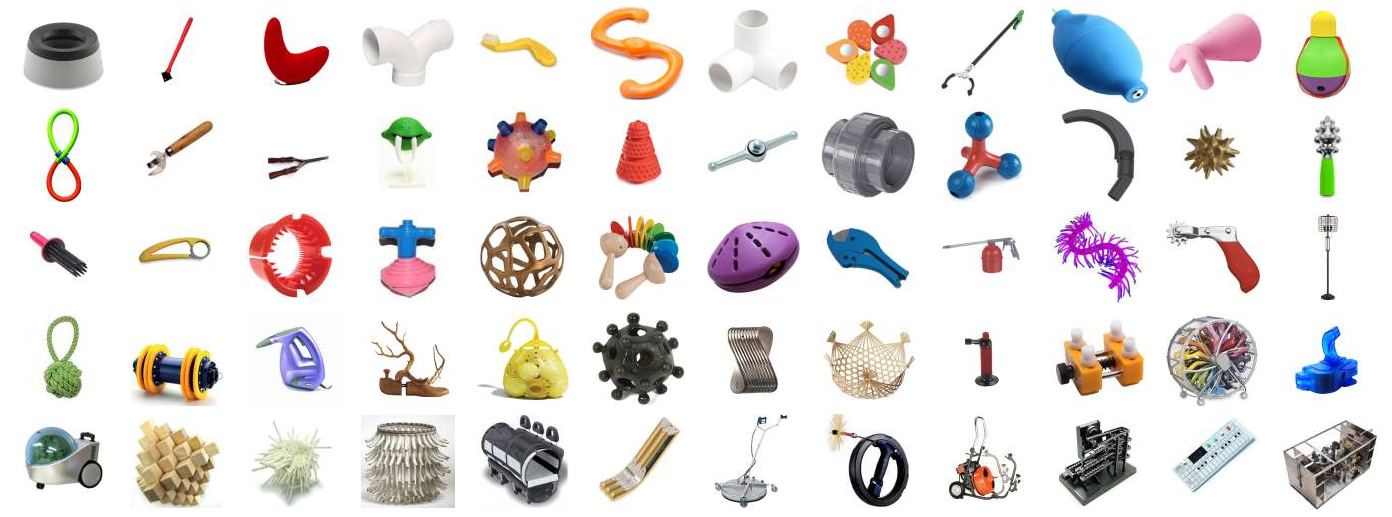
\includegraphics[width = 1\linewidth]{figs/realobjs.pdf}
%\end{center}
%\vspace{-.24em}
%\caption{Object stimuli used in the Experiment. The objects are sorted from least complex (top left) to most complex (bottom right) based on the complexity norms in Chapter 2. Each row corresponds to a quintile.}
%\label{fig:objs}
%\vspace{-1em}
%\end{figure}



In the first generation, the words were composed of randomly concatenated syllables of 3, 5, 7, 9 or 11 characters in length. Words contained CV syllables and ended in a consonant (e.g., ``gan," ``panur," ``pugimog," ``tigadogog," and ``mogonokigan"). Each participant saw 2 words of each length. The assignment of word lengths to objects was arbitrary.

Participants in Generation 2 were yoked with a participant from this first generation. This meant a participant in Generation 2 would see the exact same set of pictures as the yoked participant from Generation 1, but would learn the labels for those objects that the yoked participant had produced in the testing phase of Generation 1. Order of presentation in the training phase was randomized across generations. We iterated this procedure for a total of 7 generations.

\subsubsection{Procedure} 


Participants viewed a webpage that informed them they would be learning the names of 10 objects in an alien language. They were told they would see the names for each object four times and then their memory for the name of each object would be tested. Participants next viewed a screen displaying an object and the associated label below it. Participants pressed the space bar to advance to the next picture. Each picture-word pair was shown four times. 

In the test phase, participants saw a screen with a picture and were asked to type the learned label in a text box below the picture. Memory for each of the 10 objects was tested.

\subsection{Results}



We conducted three analyses exploring how iterated learning influenced the structure of lexicons.\footnote{All code and data for the paper are available at \url{http://github.com/mllewis/iteratedRC}.} In Analysis 1, we examined the evolution of lexical forms. In Analysis  2, we considered the relationship between word length and referent complexity. This was the key analysis because it allowed us to test for a complexity bias in the lexicon and how this bias changed over time. Finally, in Analysis  3, we conducted a post-hoc analysis to understand the source of variability in cross-generational change in complexity bias across chains.


% latex table generated in R 3.1.0 by xtable 1.7-4 package
% Fri Jan 23 11:41:41 2015
\begin{table*}[t]
\centering
%\begin{tabular}{r|llllllllll}
%\begin{tabular}{r| |l | l |l |l |l|l |l |l|l| l}
\begin{tabular}{c rrrrrr}
\hline
 %\multicolumn{11}{c}{Object} 
 %\hline

% \rule{0pt}{2ex}    
& 1 (Q1)  & 2 (Q2) & 3 (Q3) &4 (Q4) &  5 (Q5)  \\ 
 \hline
    {\it Gen.\ 0} & damitobup & nid & dunobax &  bipag &  nimimog \\ 
   {\it Gen.\ 1}& nilobup & nid & dunobug& bipag  & nimimog \\ 
    {\it Gen.\ 2} & nilobup & nid &  dunbug & bippenbog &  nimobop  \\ 
  {\it Gen.\ 3} & nilobop & nid & rdabop &  buttenbug &  nimobop \\ 
   {\it Gen.\ 4} & nilobop & nid &  dabop & buttenbop &  nimbobop \\ 
    {\it Gen.\ 5}  & nilop & nir &  dabop &  bittenbop  & nilobop \\ 
   {\it Gen.\ 6}& nilop & nir & dabop &  bittenbop &nilop \\
   {\it Gen.\ 7}& nilop &  hir &  dabog &  bittenbop &nilop  \\ 
\hline
\end{tabular}
\caption{A representative language chain. Words are presented for a sample of 5 objects across 7 generations and the initial input language. The complexity quintile of the object is noted parenthetically. Across generations, words tend to get shorter, less unique, and phonotactically more probable. Words also become more likely to be remembered accurately.}
\label{tab:ex}
\end{table*}
\normalsize

\begin{figure}[t!]
\begin{center}
\includegraphics[scale = .3]{figs/Plot1.pdf}
\end{center}
\vspace{-.5em}
\caption{Changes in lexical features across generations. Error bars represent 95\% confidence intervals computed via non-parametric bootstrap across chains.}
\label{fig:length}
\vspace{-1em}
\end{figure}





Across generations, 1\% of object labels were excluded because they contained more than one word or no word was produced. In these cases, the object was re-assigned a label from a different participant in that generation. The label was selected from a trial that had both the same initial word length and an object from the same quintile. 

\subsubsection{Analysis 1: Word forms}



Table \ref{tab:ex} presents a representative language chain. We analyzed four features of the lexical forms, averaging across each of the 50 chains at each generation: mean word length, number of unique words, transition probability, and accuracy. We also analyzed the degree of lexical change at each generation using the Levenshtein edit distance metric.

Across generations, mean word length decreased from an initial length of 7 characters to 5.22 characters in Generation 7 ($SD= 2.25$; $r=-0.22, p<.0001$; Figure\ \ref{fig:length}a). The number of unique words also decreased across generations ($r=-0.35, p<.0001$; Figure\ \ref{fig:length}b). Lexicons tended to reduce in size by mapping the same word to multiple objects (e.g.,\ in the chain presented in Table \ref{tab:ex}, ``nilop'' refers to both Objects 1 and 9).




Third, the mean orthographic transition probability of each word increased across generations ($r=.52, p<.0001$; Figure\ \ref{fig:length}c). Transition probabilities were calculated based on the set of words in the lexicon for a particular participant at a particular generation. This finding suggests that lexicons became more phonotactically structured across time. We also calculated the mean transition probability of each word using English transitions. Probabilities were estimated via orthographic bigrams from the Google Books corpus \cite{norvig}. In this analysis, the mean English transition probability of each word also increased across generations ($r=0.18$, $p <.001$), suggesting that the orthographic structure of individual words became somewhat more similar to English across generations. % vowel/consonants


Fourth, we found that participants became more accurate in recall across generations ($r=.46, p<.0001$; Figure\ \ref{fig:length}d). To examine the relationship between accuracy and word forms, we constructed a logistic mixed-effects model predicting accuracy with word length, word uniqueness, and transition probability.\footnote{The model specification was as follows: \texttt{accuracy $\sim$ guessed label length~$\times$~transition probability~$\times$~ uniqueness + (guessed label length~\textbar~subject) +  (1~\textbar~chain)}.} Only word length was a reliable predictor of accuracy ($\beta=1.21$, $p <.0001$), suggesting that perhaps the increase in accuracy across generations was due to the shorter length of the words in these languages. %phonotactics is highly collinear with number of unique words so can't put in both predictors [f

\begin{figure}[t!]
\begin{center}
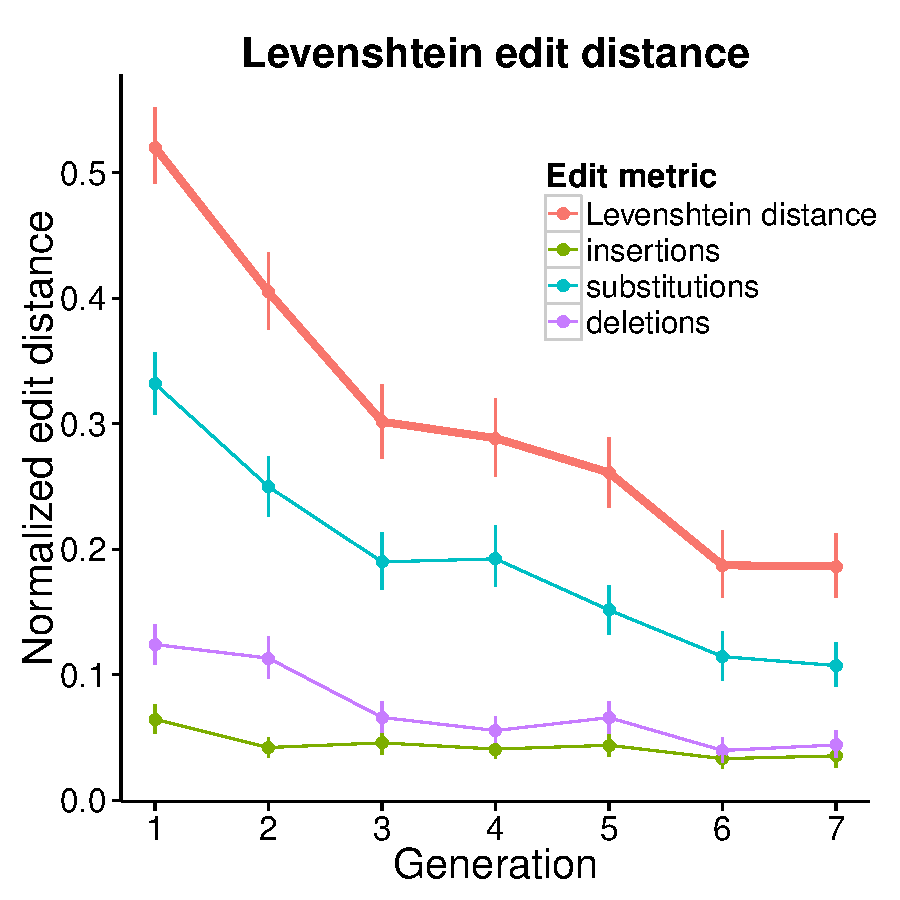
\includegraphics[width = .6\linewidth]{figs/lev.pdf}
\end{center}
\caption{Edit distance across generations, normalized by length of the longest word (guessed word vs.\ actual word). The top line shows the Levenshtein edit distance. The lines below reflect the components of this metric (substitutions, deletions, and insertions). Error bars represent 95\% confidence intervals computed via non-parametric bootstrap across chains. Number of edits decreased across generations.}
\label{fig:lev}
\end{figure}



%To examine the relationship between accuracy and features of the lexical forms, we constructed an additive linear model predicting accuracy with word length, number of unique words, and mean bigram probability. Both word length ($\beta=-0.25$, $p <.0001$) and number of unique words ($\beta=-0.28$, $p <.0001$) were reliable predictors of accuracy. This suggests that the increase in accuracy across generations was related to these changes in the features of the lexicon.

Finally, we analyzed word changes across generations using Levenshtein edit distance. This measure provides a formal metric of the similarity between two strings. Levenshtein edit distance is computed by counting the minimum number of character edits necessary to transform one word into another. For example, the edit distance from ``can" to ``cat" is 1 (1 substitution), while the edit distance from ``can" to ``calculator" is 8 (1 substitution and 7 insertions). For each word, we calculated a normalized measure by dividing the edit distance between the guessed word and the actual word by the length of the longest of the two. This normalized measure controlled for the decrease in word length across generations.  Across generations, the normalized edit distance decreased ($r=-.30, p<.0001$; Figure\ \ref{fig:lev}). This decreasing trend also held for each of the components of the Levenshtein metric: number of deletions ($r=-.18, p<.0001$), insertions ($r=-.08, p<.0001$) and substitutions ($r=-.27, p<.0001$). 

Taken together, this set of analyses points to a lexicon that is evolving to become more regular and consequently easier to learn.


%consonant/vowel analysis?

\subsubsection{Analysis 2: Complexity bias} 

In Analysis  2, we examined the relationship between changes in word length and the complexity of referents. If there is a complexity bias in the lexicon, participants should be more likely to produce longer labels for more complex referents. 

We considered two metrics of word length: Label length in characters and cumulative characters removed (CCR). CCR is calculated by subtracting the word length at a particular generation from the input generation word length. Though slightly more complex, CCR provides a length metric that controls for variability in input word length; this control is important because words varied dramatically in their initial length due to random assignment in the initial generation. We calculated $p$-values based on an empirical distribution of $r$-values, obtained by sampling from random pairings of words and objects. This was done because changes in  language forms across generations change the distribution of possible $r$-values.

\begin{figure}[t!]
\begin{center}
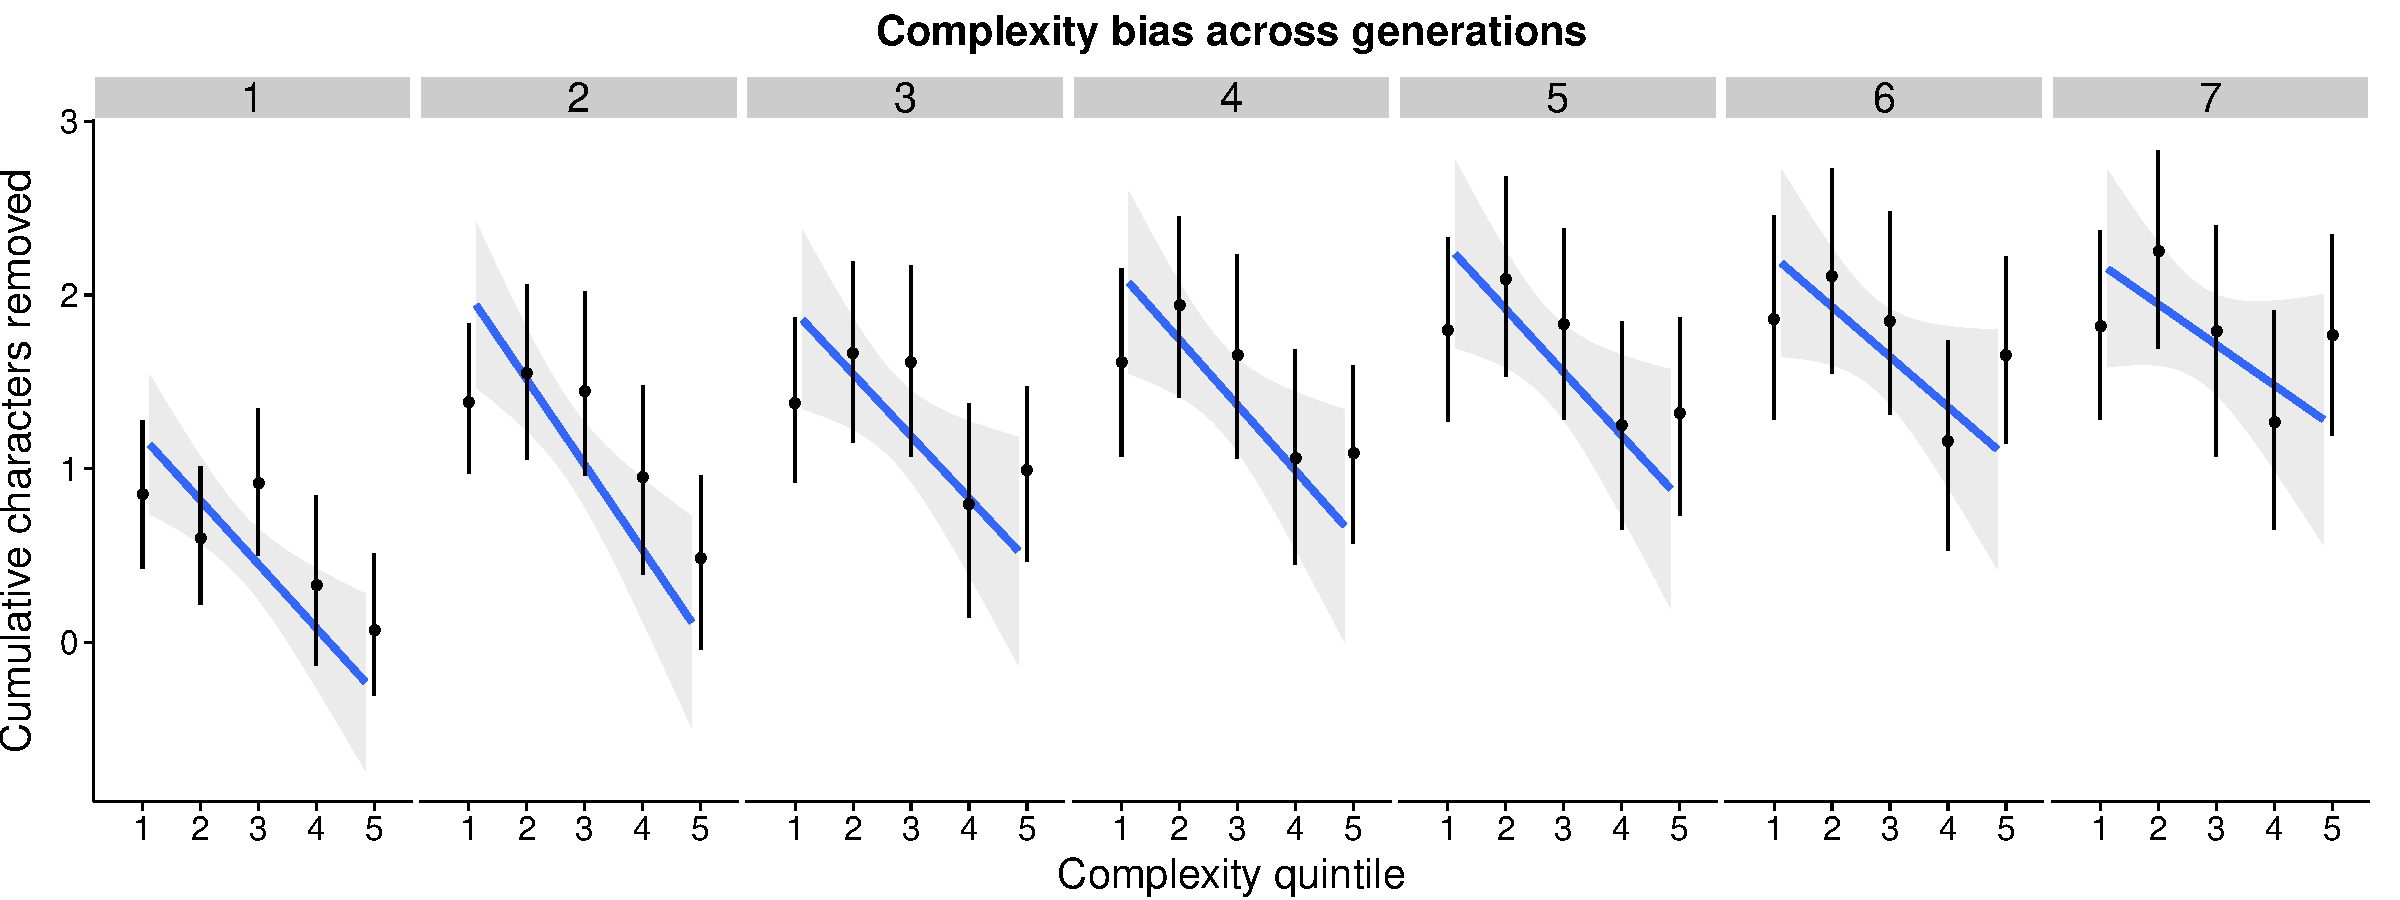
\includegraphics[scale = .38]{figs/complexity_bias.pdf}
\end{center}

\caption{Cumulative characters removed as a function of complexity across all 7 generations. Points correspond to the quintile means. Lines represent the best fitting linear model predicting word length from the complexity norm of the object. Negative slopes indicate a bias to recall longer labels for  more complex objects. Across generations, this bias decreased.}
\label{fig:cbias}
\end{figure}



Across generations, there was a reliable bias to map longer words to more complex referents across both measures of length (label length: $r=.05, p<.05$; CCR: $r=-.11, p<.0001$). Figure \ref{fig:cbias} shows CCR as a function of object complexity across generations. Qualitatively, the bias decreased across generations. However, there was high variability across chains both in the total complexity bias (label length: $SD = .27$), and in how this bias changed across generations (label length: $M = .004$; $SD = .69$).

\begin{table}[t!]

\centering
\begin{tabular}{cc|ccccccc}

\multicolumn{2}{c}{\multirow{2}{*}{}} & \multicolumn{4}{c}{Quintile  1}\\
\multicolumn{2}{c|}{}                    & 2 & 3 & 4 & 5\\ \cline{2-6}
\multirow{4}{*}{\rotatebox{90}{Quintile  2}} & 1 & 86 &  78 & 64 & 52 \\
                                      & 2 &    &   84 & 63 & 34\\
                                      & 3 &   & & 41 & 59\\
                                       & 4 &   &  &  & 58\\
                                       \vspace{-.5em}

\end{tabular}  

\caption{Contingency table of trials where participants recalled the same word for multiple objects. Columns correspond to the complexity quintile of the target object and rows correspond to the  complexity quintile of the object with the same word. The diagonal is excluded because the experimental design restricted the number of possible confusions for these cases (1 possible alternative vs.\ 2 for all other quintiles). In cases of confusions, participants tended to reuse a word from an object in a nearby quintile.}
\label{tab:confusion}
\end{table}

A number of other exploratory analyses suggest a role for complexity in language change. First, Levenshtein edit distance was systematically related to the complexity of referents: Participants were more likely to edit words referring to more complex referents ($r=.05, p<.01$). Second, there was systematicity in the kinds of errors participants  made when reusing words across multiple objects. Participants tended to reuse labels from objects of nearby quintiles (Table\ \ref{tab:confusion}), suggesting that these labels were more conceptually confusable and lead to more category-formation.

Together, this set of analyses replicates prior work suggesting a complexity bias in the lexicon: Across both measures of word length, participants tended to recall longer labels to refer to more complex referents. They were also more likely to edit words related to more complex referents and reuse labels of objects from nearby quintiles. However, an unexpected finding was the attenuation of this bias across generations. In our last analysis, we try to understand this trend.

%\begin{figure}[t]
%\begin{center}
%\includegraphics[scale = .4]{figs/confusion.pdf}
%\end{center}
%\caption{Contingency table for all trials in which participants recalled the same word for multiple referents. The diagonal is excluded because the experimental design restricted the number of possible confusions for these cases (1 possible alternative vs.\ 2 for all other quintiles). When a participant mapped the same word to a second referent, they tended to reuse a word from an object in a nearby quintile.}
%\label{fig:confusion}
%\end{figure}
% latex table generated in R 3.1.0 by xtable 1.7-4 package
% Tue Feb  3 10:17:16 2015

  
\subsubsection{Analysis  3: Relationship between change in word forms and change in complexity bias} 


\begin{figure}[t]
\begin{center}
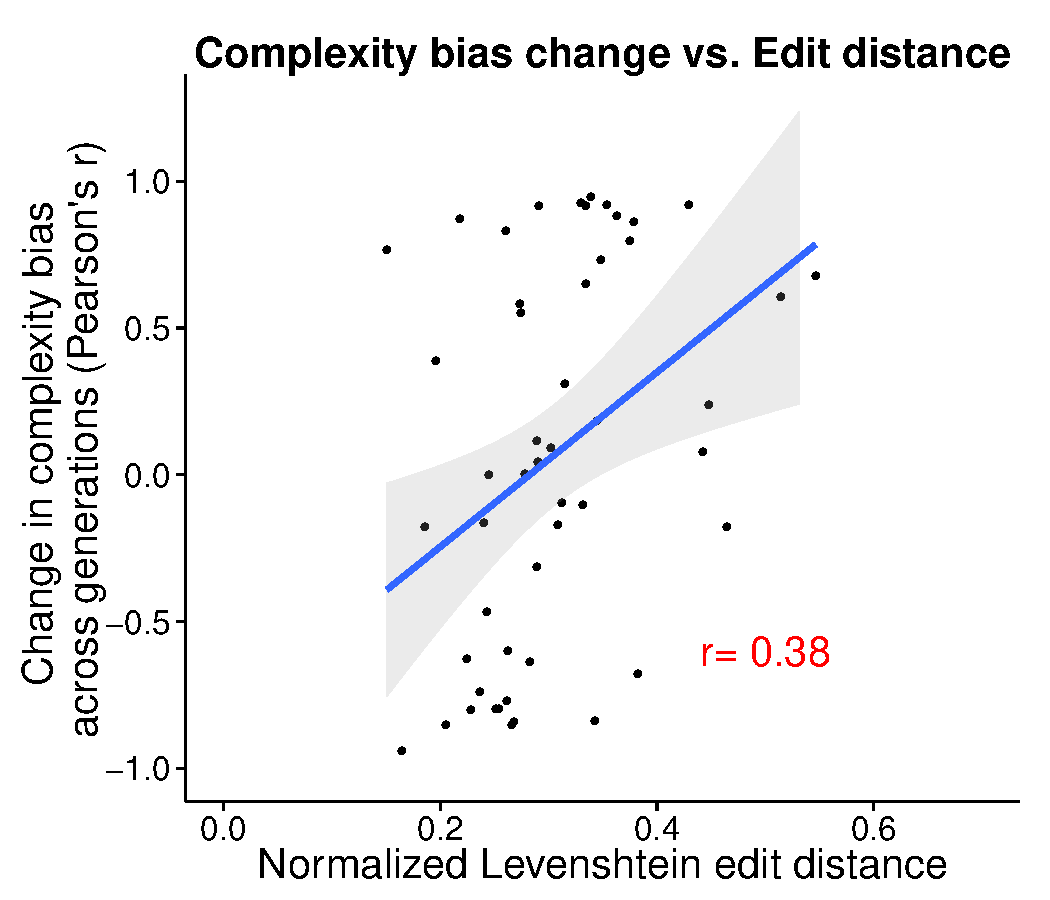
\includegraphics[width = .6\linewidth]{figs/change_plot.pdf}
\end{center}
\caption{Complexity bias as a function of the normalized Levenshtein edit distance of the chain. Complexity bias is calculated here using number of cumulative characters removed. Each point corresponds to an individual chain. Chains with greater normalized Levenshtein distances tended to show a greater increase in complexity bias across generations.}
\label{fig:levcbias}
\end{figure}



We  conducted a post-hoc exploration of the variability in the complexity bias across chains. For each chain, we quantified the complexity bias at each generation by calculating the correlation between metrics of length (label length and CCR) and the complexity norms. We then calculated the correlation between these coefficients and generation. This gave us a measure of the change in the complexity bias across generations. We considered how this change in complexity bias related to the degree of change in the forms of the lexicon. Two metrics of lexical change were analyzed: accuracy and Levenshtein edit distance. 

Chains with greater cross-generational change in lexical forms tended to show an increase in complexity bias over time. Using raw label length as the length metric, there was a reliable correlation between change in complexity bias and accuracy ($r=0.29$, $p <.05$) and between  change in complexity bias  and normalized Levenshtein edit distance ($r=-0.32$, $p =.02$). This same pattern also held for the CCR length metric (accuracy: $r=-0.37$, $p <.01$; Levenshtein: $r=0.38$, $p <.01$; Figure\ \ref{fig:levcbias}).




%%%% DISCUSSION %%%%%%
\subsection{Discussion}

In three analyses, we examined change in the structure of lexicons across generations of transmission. Analysis  1 reveals that lexical forms become simpler and more regular over time. We find that words become shorter, less unique, more phonotactically probable, and more likely to be remembered. We also find that this structure facilities memory recall: lexicons with fewer and shorter words are more likely to be remembered accurately. Analysis  2 examined the relationship between lexical forms and conceptual structure, and found that a complexity bias emerges in the lexicons. 

An unpredicted result was that the complexity bias does not strengthen across generations. Analysis  3 suggests that change in the complexity bias across generations is related to the degree of change in lexical forms in the chain: Chains with more change are more likely to show an increase in complexity bias over time. The underlying mechanism supporting this relationship is straight-forward: chains that make more errors have more opportunity to deviate from the random input mappings between words and referents. This direction of this correlation suggests that when chains do in fact deviate from these initials mappings, they do so in a systematic way. That is, they tend to deviate in a way that is more likely to map longer words onto more complex referents.

%The iterated learning paradigm provides an opportunity to examine how in-the-moment psychological pressures influence the structure of a language in aggregate, over time. We examined two aspects of this structure: lexical forms and the mappings between words and objects. We hypothesized that different psychological pressures would influence each type of structure. In the case of lexical forms, we predicted there would be a bias to simplify the language into shorter, fewer forms. In the case of word-object mappings, we predicted a bias to map longer words onto more complex meanings \cite{lewisstructure2014}. The question of interest was how these psychological pressures influenced the structure of the lexicon across generations of transmission. 

%Our findings suggest that each of these pressures may have influenced the structure of the lexicon---and critically---that they interacted with each other. 

In sum, we found both a bias to simplify the lexicon and a bias to map longer words onto more complex meanings. But these pressures appear to have pushed in opposite directions: The pressure to simplify the language leads to less variability in word length, and this reduced variability suppresses the complexity bias. If these dynamics reflect actual language evolution, however, an important question still remains---why do we in fact see a complexity bias in natural language? That is, if there is a strong pressure towards simplicity, then why does a complexity bias emerge in natural language despite this pressure? 

The Pragmatic Hypothesis suggests that this this discrepancy is due to the absence of an important feature in our task: Communication with a second interlocutor. \citeA{zipf1949human} argued that the equilibrium that emerges in the lexicon is a product of both the speaker's desire to say less and the listener's desire for a more explicit, comprehensible message. Importantly, the common desire for efficiency creates opposing pressures among interlocutors. For a speaker, the optimal solution to communication is to have a lexicon that contains a single, short word that can be used to refer to all meanings. However, for a listener, the optimal solution is to have a lexicon that maps a unique word onto every possible meaning. 

Thus, perhaps the absence of a listener pressure in our task may have lead our participants (``speakers'') to simplify the language. While our task was posed as a memory task, there was no penalty for failure to remember a form. In contrast, in a communicative task, the listener's failure to comprehend a label would have acted as an incentive for accurate reproduction, perhaps limiting the amount of compression the language would undergo.  In Study 4, we test this prediction.

%But memory limitations may also play another role in the evolution of the lexicon: by introducing variation into the representations of individual words, speakers' memory constraints allow for change. In the absence of memory constraints, speakers might simply reproduce the language as is; thus, the interaction between cognitive and communicative pressures may function to {\it facilitate} the emergence of a complexity bias. 


% However, memory limitations insert ``noise'' into the lexicon and thus create the opportunity forthe emergence and regularization of a complexity bias. 

%This synergistic relationship between memory and change is reminiscent of the ``less-is-more'' hypothesis and its descendants \cite{newport1990maturational,hudson-kam2005}, in which cognitive limitations are invoked as an important mechanism in language learning and language change. In the case of the complexity bias, these proposals make testable predictions that can be explored by extending the present paradigm into a communicative domain with varying demands on memory.
%%%%%%%%STUDY 4%%%%%%%%
\section{Study 4: Iterated learning in a communicative memory task}

%Why did the complexity bias decrease across generations? One possibility is that this discrepancy is due to the absence of an important feature in our task: communication with a second interlocutor. \citeA{horn1984} argued that the equilibrium that emerges in the lexicon is a product of both the speaker's desire to say less and the listener's desire for a more explicit, comprehensible message. Importantly, the common desire for efficiency creates opposing pressures among interlocutors. For a speaker, the optimal solution to communication is to have a lexicon that contains a single, short word that can be used to refer to all meanings. However, for a listener, the optimal solution is to have a lexicon that maps a unique word onto every possible meaning. 

%Thus, perhaps the absence of a listener pressure in our task may have lead our participants (``speakers'') to simplify the language. While our task was posed as a memory task, there was no penalty for failure to remember a form. In contrast, in a communicative task, the listener's failure to comprehend a label would have acted as an incentive for accurate reproduction, perhaps limiting the amount of compression the language would undergo. 

In Study 4 ,we adopt the paradigm from Study 3 to simulate a listener. In the Communicative Feedback, the participant is paired with a fake communicative partner who provides feedback about the guesses. We also ran a control No Feedback condition that is a near replication of Study 3. If the attenuation of the complexity bias in Study 3 is due to reduced listener demands, we expect that providing feedback will reduce  attenuation and perhaps lead to an increase in complexity bias over generations. 

\subsection{Method}

\subsubsection{Participants}
We recruited 500 participants from Amazon Mechanical Turk. Participants were randomly assigned to the No Feedback or Communicative Feedback conditions. We ran a total of  five generations with 50 participants at each generation for each condition.

\subsubsection{Stimuli}
The object and linguistic stimuli were identical to Study 3.

\subsubsection{Procedure}
The task was identical to Study 3, with the exception of the feedback. We also added a second block (where a block corresponds to a training and testing phase) so that there was greater opportunity to observe effects of the feedback. In the Communicative Feedback condition, participants were told: ``In the next part of the experiment, you will be asked to work with a partner. Your partner also learned the labels for these 10 objects. Your partner will see a display of all 10 objects. Your job is to use the words you just learned to get your partner to select one of the objects." They then were  told they were paired with another participant, and shown their screen name. After entering their response in a chat box, they received feedback from the other participant. The feedback varied as a function of the Levenshtein edit distance of the word: If the word was highly different from the target word, the  dummy-partner responded with uncertainty (``I don't know what you mean"). However, if the word was sufficiently similar (above a threshold Levenshtein value), the dummy-partner responded affirmatively (``Got it'').

\subsection{Results}

We conducted the same set of primary analyses as in Study 3: Change of word forms across generations (Analysis 1), and change in complexity bias across generations (Analysis 2). 

\subsubsection{Analysis 1: Word forms}

\begin{figure}[t!]
\begin{center}
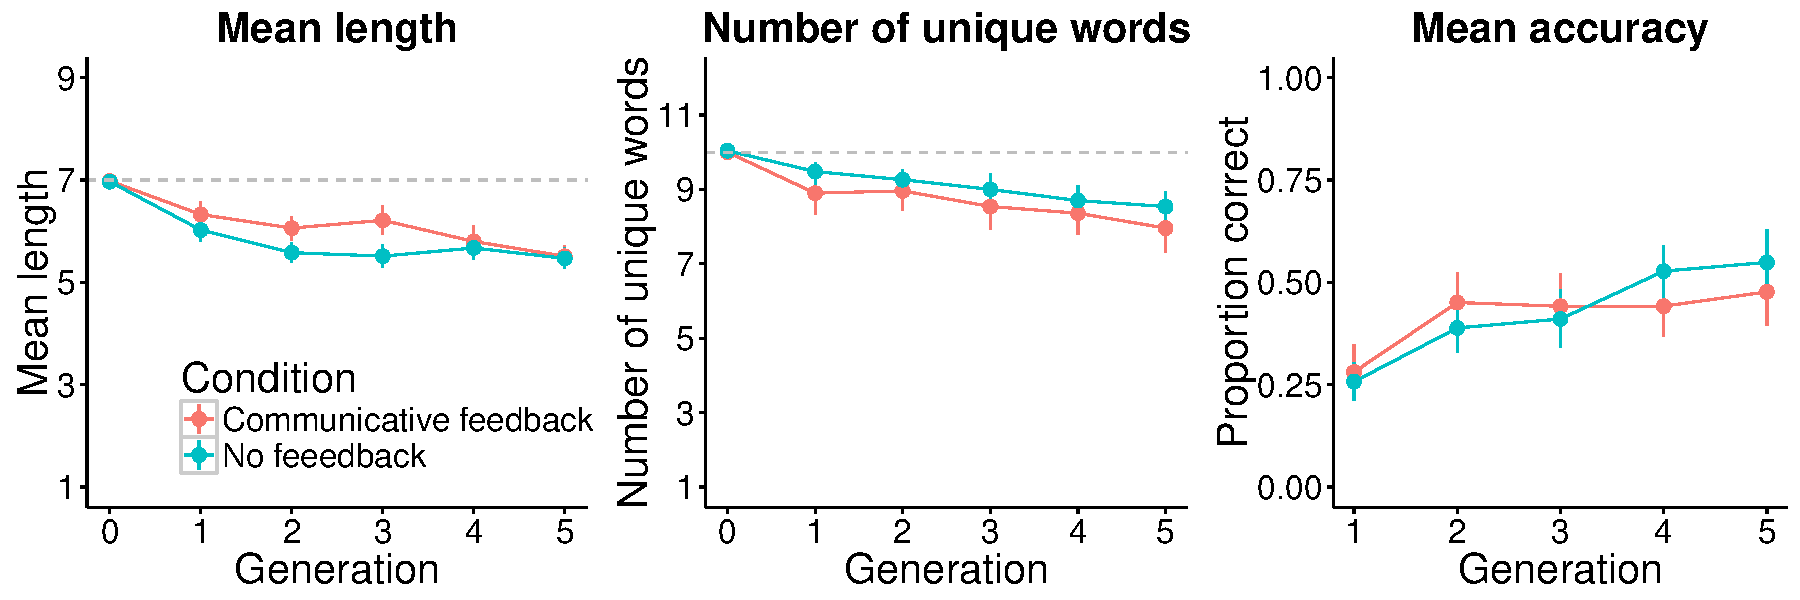
\includegraphics[scale = .5]{figs/chap4_4.pdf}
\end{center}
\caption{Changes in lexical features across generations. Error bars represent 95\% confidence intervals computed via non-parametric bootstrap across chains. }
\label{fig:length_4}
\end{figure}

As in Study 3,  mean word length and number of unique words both decreased across generations (Figure\ \ref{fig:length_4} a and b). To test for an effect of condition, we fit a mixed-effect linear model predicting word length with  condition and generation as fixed effects, and random intercepts and slopes by chain. There was a main effect of generation ($\beta=-.3$, $p <.001$). There was also an interaction with feedback condition ($\beta=-.06$, $p <.05$). This reflects the fact that word lengths decreased slower for the Communicative Feedback condition, relative to No Feedback. We then fit the same model but predicting number of unique words. There was a reliable effect of generation ($\beta=-.25$, $p <.001$), but no effect of condition.

Finally, we also found that participants became more accurate in recall across generations (Figure\ \ref{fig:length_4}c). Fitting the same model as above to predict accuracy, there was an effect of generation ($\beta=.04$, $p <.001$), and a reliable interaction between generation and condition  ($\beta=.04$, $p <.05$). This interaction reflects a small bias for participants in the Communicative Feedback condition to be more accurate in earlier generations. 

Thus, in sum, we replicate our findings from Study 3 in the No Feedback condition: Word length and number of unique words decreased across generations, while accuracy increased. In the Communicative Feedback condition, word forms decreased in length slightly slower and were initially more accurate than in the No Feedback condition. However, for the most part, we find that feedback condition did not have a substantial influence on word forms.

%However, we do not find much evidence that communicative feedback type influence the change of word forms. 
%I have run the No Feedback and Communicative Feedback condition. The No Feedback condition replicates Study 3. In the Communicative Feedback condition, mean length appears to be somewhat longer,  but the complexity bias is smaller overall and does not increase across generations.
\begin{figure}[t!]
\begin{center}
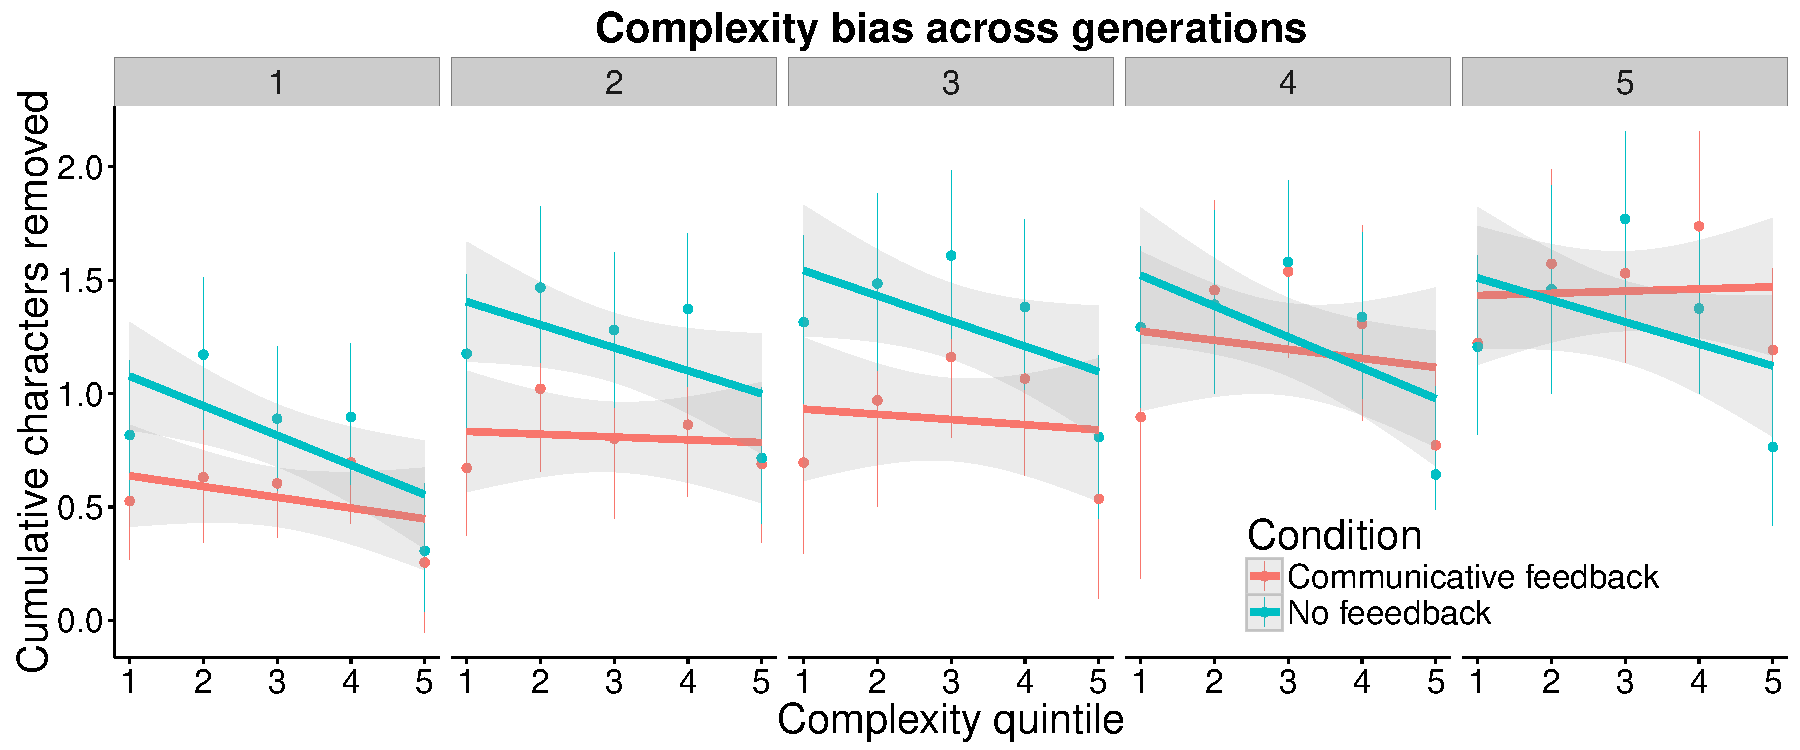
\includegraphics[scale = .5]{figs/chap4_4bias.pdf}
\end{center}
\caption{Cumulative characters removed as a function of complexity across all 5 generations. Points correspond to the quintile means. Lines represent the best fitting linear model predicting word length from the complexity norm of the object. Negative slopes indicate a bias to recall longer labels for  more complex objects. Across generations, this bias decreased, and there was no evidence to support the prediction that communicative feedback strengthened the bias.}
\label{fig:cbias4}
\end{figure}


\subsubsection{Analysis 2: Complexity bias}
In Analysis 2, we examined the key hypothesis: The magnitude of the complexity bias should be affected by feedback condition. As in Study 3, we analyzed the cumulative number of characters removed as our measure of length. For each condition, we measured the correlation between the complexity measure of the word and cumulative characters removed. Collapsing across conditions, the magnitude of the bias was larger in the No Feedback condition ($r = -0.08$), relative to the Communicative Feedback condition  ($r = -0.03$).  Figure\ \ref{fig:cbias4} shows the complexity bias across generations for each of the two conditions. Qualitatively, there is no evidence to suggest that the bias increased in the Communicative Feedback condition, as predicted by the Pragmatic Hypothesis. If anything, it appears to decrease. 

\subsection{Discussion}
The Pragmatic Hypothesis provided one possible explanation for the absence of a strengthening of the complexity bias in Study 3. In Study 4, we tested this prediction by introducing a (fake) interlocutor to give feedback to participants. However, there is no evidence to suggest that this pressure functioned to  increase the bias over time.

It is possible that this null effect is due to unusual setup of our task, such that participants did not believe the ``communicative" cover story.  A stronger test of the Pragmatic Hypothesis would therefore be to conduct the same experiment in the lab in a more realistic communicative context. Alternatively, this null effect could be because communicative pressures are not the critical pressure in decreasing word lengths in this task. The current experiment cannot distinguish between these two possibilities, but nevertheless provides some evidence against the Pragmatic Hypothesis.

\section{General Discussion }
In this chapter, we surveyed evidence relevant to four possible hypotheses about the origins of a complexity bias in natural language: The Efficient Naming Hypothesis, the Learning Hypothesis, the Memory Hypothesis, and the Pragmatic Hypothesis. In Study 1, we replicated our earlier work and found a complexity bias in a large sample of diverse languages. In Study 2, we found that children have a complexity bias in an online mapping task, and that conceptual complexity predicts the age of acquisition of a word in a child's vocabulary. In Studies 3 and 4, we found that memory errors lead to a complexity bias in an artificial language, but that this bias did not increase when a communicative partner was present.

We now have estimates of a complexity bias in natural language across three samples of words. Averaging across the seven languages described in Study 2b, we see that the magnitude of the complexity biases are remarkably comparable across a sample of seven languages, around $r = .4$ (Google: $r = .44$; Swadesh; $r = .39$;  CDI: $r = .39$). Given that all but one of these language in this subsample is from the Indo-European language family, this estimate should be interpreted cautiously. Importantly, however, we replicate our previous work pointing to a complexity bias across a range of words and languages.

Given this body of evidence, what are the most likely origins of the complexity bias in natural language? The Efficient Naming Hypothesis seems unlikely for several reasons. First, Study 1 suggests that languages have a complexity bias in a  sample of highly primitive meanings. If the Efficient Naming Hypothesis were correct, we should expect these meanings to be all assigned short words. Second, the fact that there are many unused short words in a language (e.g.\ ``dax," ``blicket," etc.) suggests that minimizing word length is not the only pressure speakers face. Indeed, there is reason to think that variability in word length is helpful for discriminating words in the cognitive system. Finally, the fact that we observe the complexity bias with novel words in word mapping tasks suggests that speakers have a cognitive representation of this bias. This cannot be explained by the Efficient Naming Hypothesis.

The evidence supporting the Pragmatic Hypothesis is also limited. In Study 4, we find no evidence that the presence of a communicative partner increased the magnitude of the bias. However, it seems possible that participants were not persuaded by the communicative cover story, though the slight difference in mean lengths across generations is some evidence against this. On the other hand, the pragmatic explanation provides a parsimonious account of children's failures in Study 1a. As has been shown in other work, young children often fail at pragmatic reasoning without sufficient contextual support. This account might then explain why the younger children in our sample, the three- and four-year-olds, failed to show a complexity bias in an online task. 

The Learning and Memory Hypotheses thus seem most likely. The fact that there is a complexity bias in children's vocabulary and that conceptual complexity predicts acquisition is suggestive that learning pressures my lead to a complexity bias in the lexicon. In addition, the fact that we see a complexity bias emerge from memory errors suggests this bias might by influenced by in-the-moment cognitive pressures. Together, these two sets of results suggest that speakers may be influenced by iconicity.

The primary focus of this chapter has been to provide an account for the complexity bias present in natural language, but a related datum is the complexity bias observed in-the-moment of language use in novel word mapping tasks. Findings from these experiments suggest that the bias is not only present in language, but is also represented in the minds of speakers and is productive. The most parsimonious account of both data points---the complexity bias in natural language and the complexity bias in novel word mapping tasks---would appeal to the same mechanism. If the Learning and Memory Hypotheses are correct, this is might mean that participants in the online mapping task are relying on the principle of iconicity to guess the meaning of the word. 

However, this need not necessarily be the case: The in-the-moment bias in the novel word mapping task could be the product of a generalization from the bias in natural language. This is a difficult possibility to explore, but one prediction of this hypothesis is that the bias should get larger as children learn more words and thus have greater evidence and certainty about the bias in natural language. The fact that the bias appears to get larger with development in Study 2a is some evidence in support of this possibility. Alternatively, the Learning and Memory Hypotheses could be the correct explanation for the bias in natural language, but participants could  be relying on pragmatic reasoning in the novel word mapping tasks.  While less parsimonious than the other accounts, this alternative is nonetheless consistent with the current body of evidence.

In conclusion, on the basis of these four studies, the most likely accounts of the complexity bias in natural language are the Learning and Memory Hypotheses: Children are biased to learn words consistent with a complexity bias, and speakers make memory errors consistent with a complexity bias. Over time, these pressures at shorter timescales lead to a bias in natural language at the language evolution timescale. The Pragmatic Hypothesis remains possible, though less likely, and more realistic communicative contexts are necessary to  definitely rule out this hypothesis.

%About .27 vs. .48



%An open question from this work is where an in-the-moment bias might originate from. Parsimony.
%
%talk about in the moment bias  lexical bias vs. (e.g. overhyopthesis, compare effect sizes) - again, not mutually exclusive, parsimony

%\subsection{naming hypothesis}
%Under this hypothesis, there are several ways to account for a pragmatic in-the-moment complexity bias. One possibility is that the lexical bias and the in-the-moment bias are the result of independent causal processes: the lexical bias may be the result of an efficient naming strategy, while the in-the-moment complexity bias may be the product of  general pragmatic reasoning. 

%An alternative possibility is that  the  in-the-moment bias emerged from a generalization, or overhypothesis \cite{kemp2007}, based on observations about the lexicon. That is, given experience with a lexicon that contains a regularity to map longer words to more complex meanings, learners might have induced a complexity  regularity about the lexicon. Thus, when faced with a novel word, speakers might apply this bias as a probabilistic heuristic about the meaning of the word. An overhypothesis account of the behavioral data has the advantage that it is able to account for the development  in an in-the-moment complexity bias in preschoolers. Under this account, preschoolers might not show this behavioral bias because they have not yet observed enough data to induce a complexity overhypothesis.



